
% Default to the notebook output style

    


% Inherit from the specified cell style.




    
\documentclass[11pt]{article}

    
    
    \usepackage[T1]{fontenc}
    % Nicer default font (+ math font) than Computer Modern for most use cases
    \usepackage{mathpazo}

    % Basic figure setup, for now with no caption control since it's done
    % automatically by Pandoc (which extracts ![](path) syntax from Markdown).
    \usepackage{graphicx}
    % We will generate all images so they have a width \maxwidth. This means
    % that they will get their normal width if they fit onto the page, but
    % are scaled down if they would overflow the margins.
    \makeatletter
    \def\maxwidth{\ifdim\Gin@nat@width>\linewidth\linewidth
    \else\Gin@nat@width\fi}
    \makeatother
    \let\Oldincludegraphics\includegraphics
    % Set max figure width to be 80% of text width, for now hardcoded.
    \renewcommand{\includegraphics}[1]{\Oldincludegraphics[width=.8\maxwidth]{#1}}
    % Ensure that by default, figures have no caption (until we provide a
    % proper Figure object with a Caption API and a way to capture that
    % in the conversion process - todo).
    \usepackage{caption}
    \DeclareCaptionLabelFormat{nolabel}{}
    \captionsetup{labelformat=nolabel}

    \usepackage{adjustbox} % Used to constrain images to a maximum size 
    \usepackage{xcolor} % Allow colors to be defined
    \usepackage{enumerate} % Needed for markdown enumerations to work
    \usepackage{geometry} % Used to adjust the document margins
    \usepackage{amsmath} % Equations
    \usepackage{amssymb} % Equations
    \usepackage{textcomp} % defines textquotesingle
    % Hack from http://tex.stackexchange.com/a/47451/13684:
    \AtBeginDocument{%
        \def\PYZsq{\textquotesingle}% Upright quotes in Pygmentized code
    }
    \usepackage{upquote} % Upright quotes for verbatim code
    \usepackage{eurosym} % defines \euro
    \usepackage[mathletters]{ucs} % Extended unicode (utf-8) support
    \usepackage[utf8x]{inputenc} % Allow utf-8 characters in the tex document
    \usepackage{fancyvrb} % verbatim replacement that allows latex
    \usepackage{grffile} % extends the file name processing of package graphics 
                         % to support a larger range 
    % The hyperref package gives us a pdf with properly built
    % internal navigation ('pdf bookmarks' for the table of contents,
    % internal cross-reference links, web links for URLs, etc.)
    \usepackage{hyperref}
    \usepackage{longtable} % longtable support required by pandoc >1.10
    \usepackage{booktabs}  % table support for pandoc > 1.12.2
    \usepackage[inline]{enumitem} % IRkernel/repr support (it uses the enumerate* environment)
    \usepackage[normalem]{ulem} % ulem is needed to support strikethroughs (\sout)
                                % normalem makes italics be italics, not underlines
    

    
    
    % Colors for the hyperref package
    \definecolor{urlcolor}{rgb}{0,.145,.698}
    \definecolor{linkcolor}{rgb}{.71,0.21,0.01}
    \definecolor{citecolor}{rgb}{.12,.54,.11}

    % ANSI colors
    \definecolor{ansi-black}{HTML}{3E424D}
    \definecolor{ansi-black-intense}{HTML}{282C36}
    \definecolor{ansi-red}{HTML}{E75C58}
    \definecolor{ansi-red-intense}{HTML}{B22B31}
    \definecolor{ansi-green}{HTML}{00A250}
    \definecolor{ansi-green-intense}{HTML}{007427}
    \definecolor{ansi-yellow}{HTML}{DDB62B}
    \definecolor{ansi-yellow-intense}{HTML}{B27D12}
    \definecolor{ansi-blue}{HTML}{208FFB}
    \definecolor{ansi-blue-intense}{HTML}{0065CA}
    \definecolor{ansi-magenta}{HTML}{D160C4}
    \definecolor{ansi-magenta-intense}{HTML}{A03196}
    \definecolor{ansi-cyan}{HTML}{60C6C8}
    \definecolor{ansi-cyan-intense}{HTML}{258F8F}
    \definecolor{ansi-white}{HTML}{C5C1B4}
    \definecolor{ansi-white-intense}{HTML}{A1A6B2}

    % commands and environments needed by pandoc snippets
    % extracted from the output of `pandoc -s`
    \providecommand{\tightlist}{%
      \setlength{\itemsep}{0pt}\setlength{\parskip}{0pt}}
    \DefineVerbatimEnvironment{Highlighting}{Verbatim}{commandchars=\\\{\}}
    % Add ',fontsize=\small' for more characters per line
    \newenvironment{Shaded}{}{}
    \newcommand{\KeywordTok}[1]{\textcolor[rgb]{0.00,0.44,0.13}{\textbf{{#1}}}}
    \newcommand{\DataTypeTok}[1]{\textcolor[rgb]{0.56,0.13,0.00}{{#1}}}
    \newcommand{\DecValTok}[1]{\textcolor[rgb]{0.25,0.63,0.44}{{#1}}}
    \newcommand{\BaseNTok}[1]{\textcolor[rgb]{0.25,0.63,0.44}{{#1}}}
    \newcommand{\FloatTok}[1]{\textcolor[rgb]{0.25,0.63,0.44}{{#1}}}
    \newcommand{\CharTok}[1]{\textcolor[rgb]{0.25,0.44,0.63}{{#1}}}
    \newcommand{\StringTok}[1]{\textcolor[rgb]{0.25,0.44,0.63}{{#1}}}
    \newcommand{\CommentTok}[1]{\textcolor[rgb]{0.38,0.63,0.69}{\textit{{#1}}}}
    \newcommand{\OtherTok}[1]{\textcolor[rgb]{0.00,0.44,0.13}{{#1}}}
    \newcommand{\AlertTok}[1]{\textcolor[rgb]{1.00,0.00,0.00}{\textbf{{#1}}}}
    \newcommand{\FunctionTok}[1]{\textcolor[rgb]{0.02,0.16,0.49}{{#1}}}
    \newcommand{\RegionMarkerTok}[1]{{#1}}
    \newcommand{\ErrorTok}[1]{\textcolor[rgb]{1.00,0.00,0.00}{\textbf{{#1}}}}
    \newcommand{\NormalTok}[1]{{#1}}
    
    % Additional commands for more recent versions of Pandoc
    \newcommand{\ConstantTok}[1]{\textcolor[rgb]{0.53,0.00,0.00}{{#1}}}
    \newcommand{\SpecialCharTok}[1]{\textcolor[rgb]{0.25,0.44,0.63}{{#1}}}
    \newcommand{\VerbatimStringTok}[1]{\textcolor[rgb]{0.25,0.44,0.63}{{#1}}}
    \newcommand{\SpecialStringTok}[1]{\textcolor[rgb]{0.73,0.40,0.53}{{#1}}}
    \newcommand{\ImportTok}[1]{{#1}}
    \newcommand{\DocumentationTok}[1]{\textcolor[rgb]{0.73,0.13,0.13}{\textit{{#1}}}}
    \newcommand{\AnnotationTok}[1]{\textcolor[rgb]{0.38,0.63,0.69}{\textbf{\textit{{#1}}}}}
    \newcommand{\CommentVarTok}[1]{\textcolor[rgb]{0.38,0.63,0.69}{\textbf{\textit{{#1}}}}}
    \newcommand{\VariableTok}[1]{\textcolor[rgb]{0.10,0.09,0.49}{{#1}}}
    \newcommand{\ControlFlowTok}[1]{\textcolor[rgb]{0.00,0.44,0.13}{\textbf{{#1}}}}
    \newcommand{\OperatorTok}[1]{\textcolor[rgb]{0.40,0.40,0.40}{{#1}}}
    \newcommand{\BuiltInTok}[1]{{#1}}
    \newcommand{\ExtensionTok}[1]{{#1}}
    \newcommand{\PreprocessorTok}[1]{\textcolor[rgb]{0.74,0.48,0.00}{{#1}}}
    \newcommand{\AttributeTok}[1]{\textcolor[rgb]{0.49,0.56,0.16}{{#1}}}
    \newcommand{\InformationTok}[1]{\textcolor[rgb]{0.38,0.63,0.69}{\textbf{\textit{{#1}}}}}
    \newcommand{\WarningTok}[1]{\textcolor[rgb]{0.38,0.63,0.69}{\textbf{\textit{{#1}}}}}
    
    
    % Define a nice break command that doesn't care if a line doesn't already
    % exist.
    \def\br{\hspace*{\fill} \\* }
    % Math Jax compatability definitions
    \def\gt{>}
    \def\lt{<}
    % Document parameters
    \title{jz2977\_hw4}
    
    
    

    % Pygments definitions
    
\makeatletter
\def\PY@reset{\let\PY@it=\relax \let\PY@bf=\relax%
    \let\PY@ul=\relax \let\PY@tc=\relax%
    \let\PY@bc=\relax \let\PY@ff=\relax}
\def\PY@tok#1{\csname PY@tok@#1\endcsname}
\def\PY@toks#1+{\ifx\relax#1\empty\else%
    \PY@tok{#1}\expandafter\PY@toks\fi}
\def\PY@do#1{\PY@bc{\PY@tc{\PY@ul{%
    \PY@it{\PY@bf{\PY@ff{#1}}}}}}}
\def\PY#1#2{\PY@reset\PY@toks#1+\relax+\PY@do{#2}}

\expandafter\def\csname PY@tok@w\endcsname{\def\PY@tc##1{\textcolor[rgb]{0.73,0.73,0.73}{##1}}}
\expandafter\def\csname PY@tok@c\endcsname{\let\PY@it=\textit\def\PY@tc##1{\textcolor[rgb]{0.25,0.50,0.50}{##1}}}
\expandafter\def\csname PY@tok@cp\endcsname{\def\PY@tc##1{\textcolor[rgb]{0.74,0.48,0.00}{##1}}}
\expandafter\def\csname PY@tok@k\endcsname{\let\PY@bf=\textbf\def\PY@tc##1{\textcolor[rgb]{0.00,0.50,0.00}{##1}}}
\expandafter\def\csname PY@tok@kp\endcsname{\def\PY@tc##1{\textcolor[rgb]{0.00,0.50,0.00}{##1}}}
\expandafter\def\csname PY@tok@kt\endcsname{\def\PY@tc##1{\textcolor[rgb]{0.69,0.00,0.25}{##1}}}
\expandafter\def\csname PY@tok@o\endcsname{\def\PY@tc##1{\textcolor[rgb]{0.40,0.40,0.40}{##1}}}
\expandafter\def\csname PY@tok@ow\endcsname{\let\PY@bf=\textbf\def\PY@tc##1{\textcolor[rgb]{0.67,0.13,1.00}{##1}}}
\expandafter\def\csname PY@tok@nb\endcsname{\def\PY@tc##1{\textcolor[rgb]{0.00,0.50,0.00}{##1}}}
\expandafter\def\csname PY@tok@nf\endcsname{\def\PY@tc##1{\textcolor[rgb]{0.00,0.00,1.00}{##1}}}
\expandafter\def\csname PY@tok@nc\endcsname{\let\PY@bf=\textbf\def\PY@tc##1{\textcolor[rgb]{0.00,0.00,1.00}{##1}}}
\expandafter\def\csname PY@tok@nn\endcsname{\let\PY@bf=\textbf\def\PY@tc##1{\textcolor[rgb]{0.00,0.00,1.00}{##1}}}
\expandafter\def\csname PY@tok@ne\endcsname{\let\PY@bf=\textbf\def\PY@tc##1{\textcolor[rgb]{0.82,0.25,0.23}{##1}}}
\expandafter\def\csname PY@tok@nv\endcsname{\def\PY@tc##1{\textcolor[rgb]{0.10,0.09,0.49}{##1}}}
\expandafter\def\csname PY@tok@no\endcsname{\def\PY@tc##1{\textcolor[rgb]{0.53,0.00,0.00}{##1}}}
\expandafter\def\csname PY@tok@nl\endcsname{\def\PY@tc##1{\textcolor[rgb]{0.63,0.63,0.00}{##1}}}
\expandafter\def\csname PY@tok@ni\endcsname{\let\PY@bf=\textbf\def\PY@tc##1{\textcolor[rgb]{0.60,0.60,0.60}{##1}}}
\expandafter\def\csname PY@tok@na\endcsname{\def\PY@tc##1{\textcolor[rgb]{0.49,0.56,0.16}{##1}}}
\expandafter\def\csname PY@tok@nt\endcsname{\let\PY@bf=\textbf\def\PY@tc##1{\textcolor[rgb]{0.00,0.50,0.00}{##1}}}
\expandafter\def\csname PY@tok@nd\endcsname{\def\PY@tc##1{\textcolor[rgb]{0.67,0.13,1.00}{##1}}}
\expandafter\def\csname PY@tok@s\endcsname{\def\PY@tc##1{\textcolor[rgb]{0.73,0.13,0.13}{##1}}}
\expandafter\def\csname PY@tok@sd\endcsname{\let\PY@it=\textit\def\PY@tc##1{\textcolor[rgb]{0.73,0.13,0.13}{##1}}}
\expandafter\def\csname PY@tok@si\endcsname{\let\PY@bf=\textbf\def\PY@tc##1{\textcolor[rgb]{0.73,0.40,0.53}{##1}}}
\expandafter\def\csname PY@tok@se\endcsname{\let\PY@bf=\textbf\def\PY@tc##1{\textcolor[rgb]{0.73,0.40,0.13}{##1}}}
\expandafter\def\csname PY@tok@sr\endcsname{\def\PY@tc##1{\textcolor[rgb]{0.73,0.40,0.53}{##1}}}
\expandafter\def\csname PY@tok@ss\endcsname{\def\PY@tc##1{\textcolor[rgb]{0.10,0.09,0.49}{##1}}}
\expandafter\def\csname PY@tok@sx\endcsname{\def\PY@tc##1{\textcolor[rgb]{0.00,0.50,0.00}{##1}}}
\expandafter\def\csname PY@tok@m\endcsname{\def\PY@tc##1{\textcolor[rgb]{0.40,0.40,0.40}{##1}}}
\expandafter\def\csname PY@tok@gh\endcsname{\let\PY@bf=\textbf\def\PY@tc##1{\textcolor[rgb]{0.00,0.00,0.50}{##1}}}
\expandafter\def\csname PY@tok@gu\endcsname{\let\PY@bf=\textbf\def\PY@tc##1{\textcolor[rgb]{0.50,0.00,0.50}{##1}}}
\expandafter\def\csname PY@tok@gd\endcsname{\def\PY@tc##1{\textcolor[rgb]{0.63,0.00,0.00}{##1}}}
\expandafter\def\csname PY@tok@gi\endcsname{\def\PY@tc##1{\textcolor[rgb]{0.00,0.63,0.00}{##1}}}
\expandafter\def\csname PY@tok@gr\endcsname{\def\PY@tc##1{\textcolor[rgb]{1.00,0.00,0.00}{##1}}}
\expandafter\def\csname PY@tok@ge\endcsname{\let\PY@it=\textit}
\expandafter\def\csname PY@tok@gs\endcsname{\let\PY@bf=\textbf}
\expandafter\def\csname PY@tok@gp\endcsname{\let\PY@bf=\textbf\def\PY@tc##1{\textcolor[rgb]{0.00,0.00,0.50}{##1}}}
\expandafter\def\csname PY@tok@go\endcsname{\def\PY@tc##1{\textcolor[rgb]{0.53,0.53,0.53}{##1}}}
\expandafter\def\csname PY@tok@gt\endcsname{\def\PY@tc##1{\textcolor[rgb]{0.00,0.27,0.87}{##1}}}
\expandafter\def\csname PY@tok@err\endcsname{\def\PY@bc##1{\setlength{\fboxsep}{0pt}\fcolorbox[rgb]{1.00,0.00,0.00}{1,1,1}{\strut ##1}}}
\expandafter\def\csname PY@tok@kc\endcsname{\let\PY@bf=\textbf\def\PY@tc##1{\textcolor[rgb]{0.00,0.50,0.00}{##1}}}
\expandafter\def\csname PY@tok@kd\endcsname{\let\PY@bf=\textbf\def\PY@tc##1{\textcolor[rgb]{0.00,0.50,0.00}{##1}}}
\expandafter\def\csname PY@tok@kn\endcsname{\let\PY@bf=\textbf\def\PY@tc##1{\textcolor[rgb]{0.00,0.50,0.00}{##1}}}
\expandafter\def\csname PY@tok@kr\endcsname{\let\PY@bf=\textbf\def\PY@tc##1{\textcolor[rgb]{0.00,0.50,0.00}{##1}}}
\expandafter\def\csname PY@tok@bp\endcsname{\def\PY@tc##1{\textcolor[rgb]{0.00,0.50,0.00}{##1}}}
\expandafter\def\csname PY@tok@fm\endcsname{\def\PY@tc##1{\textcolor[rgb]{0.00,0.00,1.00}{##1}}}
\expandafter\def\csname PY@tok@vc\endcsname{\def\PY@tc##1{\textcolor[rgb]{0.10,0.09,0.49}{##1}}}
\expandafter\def\csname PY@tok@vg\endcsname{\def\PY@tc##1{\textcolor[rgb]{0.10,0.09,0.49}{##1}}}
\expandafter\def\csname PY@tok@vi\endcsname{\def\PY@tc##1{\textcolor[rgb]{0.10,0.09,0.49}{##1}}}
\expandafter\def\csname PY@tok@vm\endcsname{\def\PY@tc##1{\textcolor[rgb]{0.10,0.09,0.49}{##1}}}
\expandafter\def\csname PY@tok@sa\endcsname{\def\PY@tc##1{\textcolor[rgb]{0.73,0.13,0.13}{##1}}}
\expandafter\def\csname PY@tok@sb\endcsname{\def\PY@tc##1{\textcolor[rgb]{0.73,0.13,0.13}{##1}}}
\expandafter\def\csname PY@tok@sc\endcsname{\def\PY@tc##1{\textcolor[rgb]{0.73,0.13,0.13}{##1}}}
\expandafter\def\csname PY@tok@dl\endcsname{\def\PY@tc##1{\textcolor[rgb]{0.73,0.13,0.13}{##1}}}
\expandafter\def\csname PY@tok@s2\endcsname{\def\PY@tc##1{\textcolor[rgb]{0.73,0.13,0.13}{##1}}}
\expandafter\def\csname PY@tok@sh\endcsname{\def\PY@tc##1{\textcolor[rgb]{0.73,0.13,0.13}{##1}}}
\expandafter\def\csname PY@tok@s1\endcsname{\def\PY@tc##1{\textcolor[rgb]{0.73,0.13,0.13}{##1}}}
\expandafter\def\csname PY@tok@mb\endcsname{\def\PY@tc##1{\textcolor[rgb]{0.40,0.40,0.40}{##1}}}
\expandafter\def\csname PY@tok@mf\endcsname{\def\PY@tc##1{\textcolor[rgb]{0.40,0.40,0.40}{##1}}}
\expandafter\def\csname PY@tok@mh\endcsname{\def\PY@tc##1{\textcolor[rgb]{0.40,0.40,0.40}{##1}}}
\expandafter\def\csname PY@tok@mi\endcsname{\def\PY@tc##1{\textcolor[rgb]{0.40,0.40,0.40}{##1}}}
\expandafter\def\csname PY@tok@il\endcsname{\def\PY@tc##1{\textcolor[rgb]{0.40,0.40,0.40}{##1}}}
\expandafter\def\csname PY@tok@mo\endcsname{\def\PY@tc##1{\textcolor[rgb]{0.40,0.40,0.40}{##1}}}
\expandafter\def\csname PY@tok@ch\endcsname{\let\PY@it=\textit\def\PY@tc##1{\textcolor[rgb]{0.25,0.50,0.50}{##1}}}
\expandafter\def\csname PY@tok@cm\endcsname{\let\PY@it=\textit\def\PY@tc##1{\textcolor[rgb]{0.25,0.50,0.50}{##1}}}
\expandafter\def\csname PY@tok@cpf\endcsname{\let\PY@it=\textit\def\PY@tc##1{\textcolor[rgb]{0.25,0.50,0.50}{##1}}}
\expandafter\def\csname PY@tok@c1\endcsname{\let\PY@it=\textit\def\PY@tc##1{\textcolor[rgb]{0.25,0.50,0.50}{##1}}}
\expandafter\def\csname PY@tok@cs\endcsname{\let\PY@it=\textit\def\PY@tc##1{\textcolor[rgb]{0.25,0.50,0.50}{##1}}}

\def\PYZbs{\char`\\}
\def\PYZus{\char`\_}
\def\PYZob{\char`\{}
\def\PYZcb{\char`\}}
\def\PYZca{\char`\^}
\def\PYZam{\char`\&}
\def\PYZlt{\char`\<}
\def\PYZgt{\char`\>}
\def\PYZsh{\char`\#}
\def\PYZpc{\char`\%}
\def\PYZdl{\char`\$}
\def\PYZhy{\char`\-}
\def\PYZsq{\char`\'}
\def\PYZdq{\char`\"}
\def\PYZti{\char`\~}
% for compatibility with earlier versions
\def\PYZat{@}
\def\PYZlb{[}
\def\PYZrb{]}
\makeatother


    % Exact colors from NB
    \definecolor{incolor}{rgb}{0.0, 0.0, 0.5}
    \definecolor{outcolor}{rgb}{0.545, 0.0, 0.0}



    
    % Prevent overflowing lines due to hard-to-break entities
    \sloppy 
    % Setup hyperref package
    \hypersetup{
      breaklinks=true,  % so long urls are correctly broken across lines
      colorlinks=true,
      urlcolor=urlcolor,
      linkcolor=linkcolor,
      citecolor=citecolor,
      }
    % Slightly bigger margins than the latex defaults
    
    \geometry{verbose,tmargin=1in,bmargin=1in,lmargin=1in,rmargin=1in}
    
    

    \begin{document}
    
    
    \maketitle
    
    

    
    \section{Homework 4}\label{homework-4}

There are two parts of this homework. In the first part, you need to
implement the backward pass of the \textbf{fully-connected layer} and
the \textbf{convolutional layer}. In the second part, we play around
with \textbf{finetuning} and \textbf{adversarial attacks} on the neural
networks!

\begin{itemize}
\item
  \textbf{Task 1: Implement NN Layers (60 points)}

  \begin{itemize}
  \tightlist
  \item
    Implement the \texttt{backward\_pass} of fully connected layer (30
    points).
  \item
    Implement the \texttt{backward\_pass} of convolutional layer (30
    points).
  \end{itemize}
\item
  \textbf{Task 2: Fintuning and Adversarial Attacks (40 points)}

  \begin{itemize}
  \tightlist
  \item
    Implement the \texttt{train} function to complete fintuinig (20
    points, 5 points per correct label in testing).
  \item
    Adversarial attacks on 4 images of 4 classes (5 points each).
  \end{itemize}
\item
  Your job is to implement the sections marked with TODO to complete the
  tasks.
\item
  Submission

  \begin{itemize}
  \tightlist
  \item
    Please submit the notebook (ipynb and pdf) including the output of
    all cells.
  \end{itemize}
\item
  Note: Please install PyTorch on your machine by running the following
  command in the terminal:

  \begin{itemize}
  \tightlist
  \item
    \texttt{pip\ install\ -U\ torch\ torchvision}
  \item
    More guideline can be found on
    \href{https://pytorch.org/get-started/locally/}{PyTorch Official
    Website}
  \item
    Task 2 is not computational intensive so you can run it on your
    local machine's CPU.
  \item
    If you want to use GPU, try
    \href{https://colab.research.google.com/}{Google CoLab} and there
    are usually free GPUs available.
  \item
    There are some
    \href{https://towardsdatascience.com/getting-started-with-google-colab-f2fff97f594c}{tutorials}
    available on how to use Colab's GPU and have your own storage.
  \end{itemize}
\end{itemize}

    \subsection{Task 1 - Implemenet NN
Layers}\label{task-1---implemenet-nn-layers}

\subsubsection{1.1 Fully Connected Layer}\label{fully-connected-layer}

Before we get started, let's recall what happens in the forward pass of
a full-connected layer.

    \begin{Verbatim}[commandchars=\\\{\}]
{\color{incolor}In [{\color{incolor}1}]:} \PY{k+kn}{import} \PY{n+nn}{math}
        \PY{k+kn}{import} \PY{n+nn}{numpy} \PY{k}{as} \PY{n+nn}{np}
        
        \PY{k}{class} \PY{n+nc}{Linear}\PY{p}{(}\PY{p}{)}\PY{p}{:}
            \PY{l+s+sd}{\PYZdq{}\PYZdq{}\PYZdq{}A fully\PYZhy{}connected NN layer.}
        \PY{l+s+sd}{    Parameters:}
        \PY{l+s+sd}{    \PYZhy{}\PYZhy{}\PYZhy{}\PYZhy{}\PYZhy{}\PYZhy{}\PYZhy{}\PYZhy{}\PYZhy{}\PYZhy{}\PYZhy{}}
        \PY{l+s+sd}{    n\PYZus{}units: int}
        \PY{l+s+sd}{        The number of neurons in the layer.}
        \PY{l+s+sd}{    input\PYZus{}shape: tuple}
        \PY{l+s+sd}{        The expected input shape of the layer. For dense layers a single digit specifying}
        \PY{l+s+sd}{        the number of features of the input. Must be specified if it is the first layer in}
        \PY{l+s+sd}{        the network.}
        \PY{l+s+sd}{    \PYZdq{}\PYZdq{}\PYZdq{}}
            \PY{k}{def} \PY{n+nf}{\PYZus{}\PYZus{}init\PYZus{}\PYZus{}}\PY{p}{(}\PY{n+nb+bp}{self}\PY{p}{,} \PY{n}{n\PYZus{}units}\PY{p}{,} \PY{n}{input\PYZus{}shape}\PY{o}{=}\PY{k+kc}{None}\PY{p}{)}\PY{p}{:}
                \PY{c+c1}{\PYZsh{} For simplisity, we omit optimizer in our homework.}
                \PY{c+c1}{\PYZsh{} Therefore, you do not need to worry about parameter update.}
                \PY{n+nb+bp}{self}\PY{o}{.}\PY{n}{layer\PYZus{}input} \PY{o}{=} \PY{k+kc}{None}
                \PY{n+nb+bp}{self}\PY{o}{.}\PY{n}{input\PYZus{}shape} \PY{o}{=} \PY{n}{input\PYZus{}shape}
                \PY{n+nb+bp}{self}\PY{o}{.}\PY{n}{n\PYZus{}units} \PY{o}{=} \PY{n}{n\PYZus{}units}
                \PY{n+nb+bp}{self}\PY{o}{.}\PY{n}{trainable} \PY{o}{=} \PY{k+kc}{True}
                \PY{n+nb+bp}{self}\PY{o}{.}\PY{n}{W} \PY{o}{=} \PY{k+kc}{None} 
                \PY{n+nb+bp}{self}\PY{o}{.}\PY{n}{b} \PY{o}{=} \PY{k+kc}{None}
                \PY{n+nb+bp}{self}\PY{o}{.}\PY{n}{initialize}\PY{p}{(}\PY{p}{)}
        
            \PY{k}{def} \PY{n+nf}{initialize}\PY{p}{(}\PY{n+nb+bp}{self}\PY{p}{)}\PY{p}{:}
                \PY{c+c1}{\PYZsh{} Initialize the weights}
                \PY{n}{limit} \PY{o}{=} \PY{l+m+mi}{1} \PY{o}{/} \PY{n}{math}\PY{o}{.}\PY{n}{sqrt}\PY{p}{(}\PY{n+nb+bp}{self}\PY{o}{.}\PY{n}{input\PYZus{}shape}\PY{p}{[}\PY{l+m+mi}{0}\PY{p}{]}\PY{p}{)}
                \PY{n+nb+bp}{self}\PY{o}{.}\PY{n}{W}  \PY{o}{=} \PY{n}{np}\PY{o}{.}\PY{n}{random}\PY{o}{.}\PY{n}{uniform}\PY{p}{(}\PY{o}{\PYZhy{}}\PY{n}{limit}\PY{p}{,} \PY{n}{limit}\PY{p}{,} \PY{p}{(}\PY{n+nb+bp}{self}\PY{o}{.}\PY{n}{input\PYZus{}shape}\PY{p}{[}\PY{l+m+mi}{1}\PY{p}{]}\PY{p}{,} \PY{n+nb+bp}{self}\PY{o}{.}\PY{n}{n\PYZus{}units}\PY{p}{)}\PY{p}{)}
                \PY{n+nb+bp}{self}\PY{o}{.}\PY{n}{b} \PY{o}{=} \PY{n}{np}\PY{o}{.}\PY{n}{zeros}\PY{p}{(}\PY{p}{(}\PY{l+m+mi}{1}\PY{p}{,} \PY{n+nb+bp}{self}\PY{o}{.}\PY{n}{n\PYZus{}units}\PY{p}{)}\PY{p}{)}
        
            \PY{k}{def} \PY{n+nf}{forward\PYZus{}pass}\PY{p}{(}\PY{n+nb+bp}{self}\PY{p}{,} \PY{n}{inp}\PY{p}{)}\PY{p}{:}
                \PY{n+nb+bp}{self}\PY{o}{.}\PY{n}{layer\PYZus{}input} \PY{o}{=} \PY{n}{inp}
                \PY{k}{return} \PY{n}{np}\PY{o}{.}\PY{n}{dot}\PY{p}{(}\PY{n}{inp}\PY{p}{,} \PY{n+nb+bp}{self}\PY{o}{.}\PY{n}{W}\PY{p}{)} \PY{o}{+} \PY{n+nb+bp}{self}\PY{o}{.}\PY{n}{b}
\end{Verbatim}


    Below we provided some helper functions that might be useful:

    \begin{Verbatim}[commandchars=\\\{\}]
{\color{incolor}In [{\color{incolor}2}]:} \PY{k}{def} \PY{n+nf}{SE}\PY{p}{(}\PY{n}{out}\PY{p}{,} \PY{n}{target}\PY{p}{)}\PY{p}{:}
            \PY{l+s+sd}{\PYZsq{}\PYZsq{}\PYZsq{}}
        \PY{l+s+sd}{    return square error.}
        \PY{l+s+sd}{    \PYZsq{}\PYZsq{}\PYZsq{}}
            \PY{k}{return} \PY{l+m+mf}{0.5} \PY{o}{*} \PY{p}{(}\PY{n}{target} \PY{o}{\PYZhy{}} \PY{n}{out}\PY{p}{)}\PY{o}{*}\PY{o}{*}\PY{l+m+mi}{2}
        
        \PY{k}{def} \PY{n+nf}{get\PYZus{}target}\PY{p}{(}\PY{n}{inp}\PY{p}{,} \PY{n}{W}\PY{p}{,} \PY{n}{b}\PY{p}{)}\PY{p}{:}
            \PY{l+s+sd}{\PYZsq{}\PYZsq{}\PYZsq{}}
        \PY{l+s+sd}{    W and b are assumed ideal weights and bias.}
        \PY{l+s+sd}{    \PYZsq{}\PYZsq{}\PYZsq{}}
            \PY{k}{return} \PY{n}{np}\PY{o}{.}\PY{n}{dot}\PY{p}{(}\PY{n}{inp}\PY{p}{,} \PY{n}{W}\PY{p}{)} \PY{o}{+} \PY{n}{b}
        
        \PY{k}{def} \PY{n+nf}{grad\PYZus{}check}\PY{p}{(}\PY{n}{layer}\PY{p}{,} \PY{n}{inp}\PY{p}{,} \PY{n}{W}\PY{p}{,} \PY{n}{b}\PY{p}{)}\PY{p}{:}
            \PY{l+s+sd}{\PYZsq{}\PYZsq{}\PYZsq{}}
        \PY{l+s+sd}{    calculate gradient from numerical method, we compare the analytical gradient and numerical gradient.}
        \PY{l+s+sd}{    }
        \PY{l+s+sd}{    We say your calculated gradients are correct when the mean square error between }
        \PY{l+s+sd}{    standard gradient and your gradient is below some threshold.}
        \PY{l+s+sd}{    }
        \PY{l+s+sd}{    return true when gradients of W, b and inp are calculated correctly.}
        \PY{l+s+sd}{    \PYZsq{}\PYZsq{}\PYZsq{}}
            \PY{n}{res} \PY{o}{=} \PY{k+kc}{True}
            \PY{n}{target} \PY{o}{=} \PY{n}{get\PYZus{}target}\PY{p}{(}\PY{n}{inp}\PY{p}{,} \PY{n}{W}\PY{p}{,} \PY{n}{b}\PY{p}{)}
        \PY{c+c1}{\PYZsh{}     print(target.shape)}
            \PY{n}{out} \PY{o}{=} \PY{n}{layer}\PY{o}{.}\PY{n}{forward\PYZus{}pass}\PY{p}{(}\PY{n}{inp}\PY{p}{)}
            \PY{n}{y} \PY{o}{=} \PY{n}{SE}\PY{p}{(}\PY{n}{target}\PY{p}{,} \PY{n}{out}\PY{p}{)}
            \PY{n}{loss} \PY{o}{=} \PY{n}{target} \PY{o}{\PYZhy{}} \PY{n}{out}
        \PY{c+c1}{\PYZsh{}     print(loss.shape)}
            \PY{n}{accum\PYZus{}grad} \PY{o}{=} \PY{n}{layer}\PY{o}{.}\PY{n}{backward\PYZus{}pass}\PY{p}{(}\PY{n}{loss}\PY{p}{)}
            
            \PY{n}{W\PYZus{}shape} \PY{o}{=} \PY{n}{layer}\PY{o}{.}\PY{n}{W}\PY{o}{.}\PY{n}{shape}
            \PY{n}{b\PYZus{}shape} \PY{o}{=} \PY{n}{layer}\PY{o}{.}\PY{n}{b}\PY{o}{.}\PY{n}{shape}
            \PY{n}{inp\PYZus{}shape} \PY{o}{=} \PY{n}{inp}\PY{o}{.}\PY{n}{shape}
            
            \PY{n}{limit} \PY{o}{=} \PY{l+m+mf}{1e\PYZhy{}6}
            \PY{n}{threshold} \PY{o}{=} \PY{l+m+mf}{1e\PYZhy{}8} \PY{o}{*} \PY{n}{inp\PYZus{}shape}\PY{p}{[}\PY{l+m+mi}{0}\PY{p}{]}\PY{o}{*}\PY{o}{*}\PY{l+m+mi}{2}
            
            \PY{n}{W\PYZus{}diff} \PY{o}{=} \PY{n}{np}\PY{o}{.}\PY{n}{zeros}\PY{p}{(}\PY{n}{W\PYZus{}shape}\PY{p}{)}
            \PY{k}{for} \PY{n}{i} \PY{o+ow}{in} \PY{n+nb}{range}\PY{p}{(}\PY{n}{W\PYZus{}shape}\PY{p}{[}\PY{l+m+mi}{0}\PY{p}{]}\PY{p}{)}\PY{p}{:}
                \PY{n}{noise} \PY{o}{=} \PY{n}{np}\PY{o}{.}\PY{n}{random}\PY{o}{.}\PY{n}{rand}\PY{p}{(}\PY{n}{W\PYZus{}shape}\PY{p}{[}\PY{l+m+mi}{1}\PY{p}{]}\PY{p}{)} \PY{o}{*} \PY{n}{limit}
                \PY{n}{layer}\PY{o}{.}\PY{n}{W}\PY{p}{[}\PY{n}{i}\PY{p}{,}\PY{p}{:}\PY{p}{]} \PY{o}{+}\PY{o}{=} \PY{n}{noise}
                \PY{n}{out2} \PY{o}{=} \PY{n}{layer}\PY{o}{.}\PY{n}{forward\PYZus{}pass}\PY{p}{(}\PY{n}{inp}\PY{p}{)}
                \PY{n}{y2} \PY{o}{=} \PY{n}{SE}\PY{p}{(}\PY{n}{target}\PY{p}{,} \PY{n}{out2}\PY{p}{)}
        \PY{c+c1}{\PYZsh{}         print(y2.shape)}
                \PY{n}{W\PYZus{}diff}\PY{p}{[}\PY{n}{i}\PY{p}{,}\PY{p}{:}\PY{p}{]} \PY{o}{=} \PY{n}{np}\PY{o}{.}\PY{n}{sum}\PY{p}{(}\PY{n}{y} \PY{o}{\PYZhy{}} \PY{n}{y2}\PY{p}{,} \PY{n}{axis}\PY{o}{=}\PY{l+m+mi}{0}\PY{p}{)} \PY{o}{/} \PY{n}{noise}
        \PY{c+c1}{\PYZsh{}         print(W\PYZus{}diff.shape)}
                \PY{n}{layer}\PY{o}{.}\PY{n}{W}\PY{p}{[}\PY{n}{i}\PY{p}{,}\PY{p}{:}\PY{p}{]} \PY{o}{\PYZhy{}}\PY{o}{=} \PY{n}{noise}
                
            \PY{n}{res} \PY{o}{\PYZam{}}\PY{o}{=} \PY{p}{(}\PY{n}{np}\PY{o}{.}\PY{n}{sum}\PY{p}{(}\PY{p}{(}\PY{n}{W\PYZus{}diff} \PY{o}{\PYZhy{}} \PY{n}{layer}\PY{o}{.}\PY{n}{grad\PYZus{}W}\PY{p}{)}\PY{o}{*}\PY{o}{*}\PY{l+m+mi}{2}\PY{p}{)} \PY{o}{\PYZlt{}} \PY{n}{threshold}\PY{p}{)}
            
            \PY{n}{noise} \PY{o}{=} \PY{n}{np}\PY{o}{.}\PY{n}{random}\PY{o}{.}\PY{n}{rand}\PY{p}{(}\PY{o}{*}\PY{n}{b\PYZus{}shape}\PY{p}{)} \PY{o}{*} \PY{n}{limit}
            \PY{n}{layer}\PY{o}{.}\PY{n}{b} \PY{o}{+}\PY{o}{=} \PY{n}{noise}
            \PY{n}{out2} \PY{o}{=} \PY{n}{layer}\PY{o}{.}\PY{n}{forward\PYZus{}pass}\PY{p}{(}\PY{n}{inp}\PY{p}{)}
            \PY{n}{y2} \PY{o}{=} \PY{n}{SE}\PY{p}{(}\PY{n}{target}\PY{p}{,} \PY{n}{out2}\PY{p}{)}
            \PY{n}{b\PYZus{}diff} \PY{o}{=} \PY{n}{np}\PY{o}{.}\PY{n}{sum}\PY{p}{(}\PY{n}{y} \PY{o}{\PYZhy{}} \PY{n}{y2}\PY{p}{,} \PY{n}{axis}\PY{o}{=}\PY{l+m+mi}{0}\PY{p}{)} \PY{o}{/} \PY{n}{noise}
            \PY{n}{layer}\PY{o}{.}\PY{n}{b} \PY{o}{\PYZhy{}}\PY{o}{=} \PY{n}{noise}
            \PY{n}{res} \PY{o}{\PYZam{}}\PY{o}{=} \PY{p}{(}\PY{n}{np}\PY{o}{.}\PY{n}{sum}\PY{p}{(}\PY{p}{(}\PY{n}{b\PYZus{}diff} \PY{o}{\PYZhy{}} \PY{n}{layer}\PY{o}{.}\PY{n}{grad\PYZus{}b}\PY{p}{)}\PY{o}{*}\PY{o}{*}\PY{l+m+mi}{2}\PY{p}{)} \PY{o}{\PYZlt{}} \PY{n}{threshold}\PY{p}{)}
            
            \PY{n}{inp\PYZus{}diff} \PY{o}{=} \PY{n}{np}\PY{o}{.}\PY{n}{zeros}\PY{p}{(}\PY{n}{inp\PYZus{}shape}\PY{p}{)}
            \PY{k}{for} \PY{n}{j} \PY{o+ow}{in} \PY{n+nb}{range}\PY{p}{(}\PY{n}{inp\PYZus{}shape}\PY{p}{[}\PY{l+m+mi}{1}\PY{p}{]}\PY{p}{)}\PY{p}{:}
                \PY{n}{noise} \PY{o}{=} \PY{n}{np}\PY{o}{.}\PY{n}{random}\PY{o}{.}\PY{n}{rand}\PY{p}{(}\PY{n}{inp\PYZus{}shape}\PY{p}{[}\PY{l+m+mi}{0}\PY{p}{]}\PY{p}{)} \PY{o}{*} \PY{n}{limit}
                \PY{n}{inp}\PY{p}{[}\PY{p}{:}\PY{p}{,}\PY{n}{j}\PY{p}{]} \PY{o}{+}\PY{o}{=} \PY{n}{noise}
                \PY{n}{out2} \PY{o}{=} \PY{n}{layer}\PY{o}{.}\PY{n}{forward\PYZus{}pass}\PY{p}{(}\PY{n}{inp}\PY{p}{)}
                \PY{n}{y2} \PY{o}{=} \PY{n}{SE}\PY{p}{(}\PY{n}{target}\PY{p}{,} \PY{n}{out2}\PY{p}{)}
                \PY{n}{inp\PYZus{}diff}\PY{p}{[}\PY{p}{:}\PY{p}{,}\PY{n}{j}\PY{p}{]} \PY{o}{=} \PY{n}{np}\PY{o}{.}\PY{n}{sum}\PY{p}{(}\PY{n}{y} \PY{o}{\PYZhy{}} \PY{n}{y2}\PY{p}{,} \PY{n}{axis}\PY{o}{=}\PY{l+m+mi}{1}\PY{p}{)} \PY{o}{/} \PY{n}{noise}
                \PY{n}{inp}\PY{p}{[}\PY{p}{:}\PY{p}{,}\PY{n}{j}\PY{p}{]} \PY{o}{\PYZhy{}}\PY{o}{=} \PY{n}{noise}
            
            \PY{n}{res} \PY{o}{\PYZam{}}\PY{o}{=} \PY{p}{(}\PY{n}{np}\PY{o}{.}\PY{n}{sum}\PY{p}{(}\PY{p}{(}\PY{n}{inp\PYZus{}diff} \PY{o}{\PYZhy{}} \PY{n}{accum\PYZus{}grad}\PY{p}{)}\PY{o}{*}\PY{o}{*}\PY{l+m+mi}{2}\PY{p}{)} \PY{o}{\PYZlt{}} \PY{n}{threshold}\PY{p}{)} 
            
            \PY{k}{return} \PY{n}{res}
\end{Verbatim}


    \subsubsection{Implement the Backward
Pass}\label{implement-the-backward-pass}

Now you can start building your own backward function of the fully
connected layer.

    \begin{Verbatim}[commandchars=\\\{\}]
{\color{incolor}In [{\color{incolor}3}]:} \PY{k}{def} \PY{n+nf}{backward\PYZus{}pass\PYZus{}fc}\PY{p}{(}\PY{n+nb+bp}{self}\PY{p}{,} \PY{n}{accum\PYZus{}grad}\PY{p}{)}\PY{p}{:}
            \PY{l+s+sd}{\PYZsq{}\PYZsq{}\PYZsq{}}
        \PY{l+s+sd}{    TODO: Implement the backward\PYZus{}pass\PYZus{}fc here.}
        \PY{l+s+sd}{    }
        \PY{l+s+sd}{    Parameter:}
        \PY{l+s+sd}{    \PYZhy{}\PYZhy{}\PYZhy{}\PYZhy{}\PYZhy{}\PYZhy{}\PYZhy{}\PYZhy{}\PYZhy{}\PYZhy{}}
        \PY{l+s+sd}{        accum\PYZus{}grad: gradient propogated back from the next layer}
        \PY{l+s+sd}{        }
        \PY{l+s+sd}{    Return:}
        \PY{l+s+sd}{    \PYZhy{}\PYZhy{}\PYZhy{}\PYZhy{}\PYZhy{}\PYZhy{}\PYZhy{}\PYZhy{}\PYZhy{}\PYZhy{}}
        \PY{l+s+sd}{        accum\PYZus{}grad\PYZus{}result: gradient propogated back from the this layer}
        \PY{l+s+sd}{    \PYZsq{}\PYZsq{}\PYZsq{}}
            
            \PY{n+nb+bp}{self}\PY{o}{.}\PY{n}{grad\PYZus{}W} \PY{o}{=} \PY{n}{np}\PY{o}{.}\PY{n}{dot}\PY{p}{(}\PY{n+nb+bp}{self}\PY{o}{.}\PY{n}{layer\PYZus{}input}\PY{o}{.}\PY{n}{T}\PY{p}{,} \PY{n}{accum\PYZus{}grad}\PY{p}{)}
            \PY{n+nb+bp}{self}\PY{o}{.}\PY{n}{grad\PYZus{}b} \PY{o}{=} \PY{n}{np}\PY{o}{.}\PY{n}{sum}\PY{p}{(}\PY{n}{accum\PYZus{}grad}\PY{p}{,} \PY{n}{axis}\PY{o}{=}\PY{l+m+mi}{0}\PY{p}{)}
            
            \PY{n}{accum\PYZus{}grad\PYZus{}result} \PY{o}{=} \PY{n}{np}\PY{o}{.}\PY{n}{dot}\PY{p}{(}\PY{n}{accum\PYZus{}grad}\PY{p}{,} \PY{n+nb+bp}{self}\PY{o}{.}\PY{n}{W}\PY{o}{.}\PY{n}{T}\PY{p}{)}
            \PY{k}{return} \PY{n}{accum\PYZus{}grad\PYZus{}result}
\end{Verbatim}


    \subsubsection{Test your implementation}\label{test-your-implementation}

Use grad\_check to test the correctness of your backward implementation:

    \begin{Verbatim}[commandchars=\\\{\}]
{\color{incolor}In [{\color{incolor}4}]:} \PY{n}{Linear}\PY{o}{.}\PY{n}{backward\PYZus{}pass} \PY{o}{=} \PY{n}{backward\PYZus{}pass\PYZus{}fc}
        
        \PY{n}{inp} \PY{o}{=} \PY{n}{np}\PY{o}{.}\PY{n}{random}\PY{o}{.}\PY{n}{rand}\PY{p}{(}\PY{l+m+mi}{100}\PY{p}{,}\PY{l+m+mi}{3}\PY{p}{)}
        \PY{n}{layer} \PY{o}{=} \PY{n}{Linear}\PY{p}{(}\PY{l+m+mi}{2}\PY{p}{,} \PY{n}{inp}\PY{o}{.}\PY{n}{shape}\PY{p}{)}
        
        \PY{n}{W} \PY{o}{=} \PY{n}{np}\PY{o}{.}\PY{n}{random}\PY{o}{.}\PY{n}{rand}\PY{p}{(}\PY{l+m+mi}{3}\PY{p}{,}\PY{l+m+mi}{2}\PY{p}{)}
        \PY{n}{b} \PY{o}{=} \PY{n}{np}\PY{o}{.}\PY{n}{random}\PY{o}{.}\PY{n}{rand}\PY{p}{(}\PY{l+m+mi}{1}\PY{p}{,}\PY{l+m+mi}{2}\PY{p}{)}
        
        \PY{k}{if} \PY{n}{grad\PYZus{}check}\PY{p}{(}\PY{n}{layer}\PY{p}{,} \PY{n}{inp}\PY{p}{,} \PY{n}{W}\PY{p}{,} \PY{n}{b}\PY{p}{)}\PY{p}{:}
            \PY{n+nb}{print}\PY{p}{(}\PY{l+s+s2}{\PYZdq{}}\PY{l+s+s2}{[INFO] Testing Backward Pass: Pass!}\PY{l+s+s2}{\PYZdq{}}\PY{p}{)}
        \PY{k}{else}\PY{p}{:}
            \PY{n+nb}{print}\PY{p}{(}\PY{l+s+s2}{\PYZdq{}}\PY{l+s+s2}{[WARN] Testing Backward Pass: Fail!}\PY{l+s+s2}{\PYZdq{}}\PY{p}{)}
\end{Verbatim}


    \begin{Verbatim}[commandchars=\\\{\}]
[INFO] Testing Backward Pass: Pass!

    \end{Verbatim}

    \subsubsection{1.2 Convolutional Layer}\label{convolutional-layer}

Before we get started, let's recall what happens in the forward pass of
a convolutional layer.

    \begin{Verbatim}[commandchars=\\\{\}]
{\color{incolor}In [{\color{incolor}5}]:} \PY{k}{class} \PY{n+nc}{Conv2D}\PY{p}{(}\PY{p}{)}\PY{p}{:}
            \PY{l+s+sd}{\PYZdq{}\PYZdq{}\PYZdq{}A 2D Convolution Layer.}
        
        \PY{l+s+sd}{    Parameters:}
        \PY{l+s+sd}{    \PYZhy{}\PYZhy{}\PYZhy{}\PYZhy{}\PYZhy{}\PYZhy{}\PYZhy{}\PYZhy{}\PYZhy{}\PYZhy{}\PYZhy{}}
        \PY{l+s+sd}{    n\PYZus{}filters: int}
        \PY{l+s+sd}{        The number of filters that will convolve over the input matrix. The number of channels}
        \PY{l+s+sd}{        of the output shape.}
        \PY{l+s+sd}{    filter\PYZus{}shape: tuple}
        \PY{l+s+sd}{        A tuple (filter\PYZus{}height, filter\PYZus{}width).}
        \PY{l+s+sd}{    input\PYZus{}shape: tuple}
        \PY{l+s+sd}{        The shape of the expected input of the layer. (batch\PYZus{}size, channels, height, width)}
        \PY{l+s+sd}{        Only needs to be specified for first layer in the network.}
        \PY{l+s+sd}{    padding: string}
        \PY{l+s+sd}{        Either \PYZsq{}same\PYZsq{} or \PYZsq{}valid\PYZsq{}. \PYZsq{}same\PYZsq{} results in padding being added so that the output height and width}
        \PY{l+s+sd}{        matches the input height and width. For \PYZsq{}valid\PYZsq{} no padding is added.}
        \PY{l+s+sd}{        By default, we use \PYZsq{}same\PYZsq{} to test the implementation.}
        \PY{l+s+sd}{    stride: int}
        \PY{l+s+sd}{        The stride length of the filters during the convolution over the input.}
        \PY{l+s+sd}{    \PYZdq{}\PYZdq{}\PYZdq{}}
            
            \PY{k}{def} \PY{n+nf}{\PYZus{}\PYZus{}init\PYZus{}\PYZus{}}\PY{p}{(}\PY{n+nb+bp}{self}\PY{p}{,} \PY{n}{n\PYZus{}filters}\PY{p}{,} \PY{n}{filter\PYZus{}shape}\PY{p}{,} \PY{n}{input\PYZus{}shape}\PY{p}{,} \PY{n}{padding}\PY{o}{=}\PY{l+s+s1}{\PYZsq{}}\PY{l+s+s1}{same}\PY{l+s+s1}{\PYZsq{}}\PY{p}{,} \PY{n}{stride}\PY{o}{=}\PY{l+m+mi}{1}\PY{p}{)}\PY{p}{:}
                \PY{n+nb+bp}{self}\PY{o}{.}\PY{n}{n\PYZus{}filters} \PY{o}{=} \PY{n}{n\PYZus{}filters}
                \PY{n+nb+bp}{self}\PY{o}{.}\PY{n}{filter\PYZus{}shape} \PY{o}{=} \PY{n}{filter\PYZus{}shape}
                \PY{n+nb+bp}{self}\PY{o}{.}\PY{n}{padding} \PY{o}{=} \PY{n}{padding}
                \PY{n+nb+bp}{self}\PY{o}{.}\PY{n}{stride} \PY{o}{=} \PY{n}{stride}
                \PY{n+nb+bp}{self}\PY{o}{.}\PY{n}{input\PYZus{}shape} \PY{o}{=} \PY{n}{input\PYZus{}shape}
                \PY{n+nb+bp}{self}\PY{o}{.}\PY{n}{trainable} \PY{o}{=} \PY{k+kc}{True}
                \PY{n+nb+bp}{self}\PY{o}{.}\PY{n}{W} \PY{o}{=} \PY{k+kc}{None}
                \PY{n+nb+bp}{self}\PY{o}{.}\PY{n}{w0} \PY{o}{=} \PY{k+kc}{None}
                \PY{n+nb+bp}{self}\PY{o}{.}\PY{n}{initialize}\PY{p}{(}\PY{p}{)}
        
            \PY{k}{def} \PY{n+nf}{initialize}\PY{p}{(}\PY{n+nb+bp}{self}\PY{p}{)}\PY{p}{:}
                \PY{c+c1}{\PYZsh{} Initialize the weights}
                \PY{n}{filter\PYZus{}height}\PY{p}{,} \PY{n}{filter\PYZus{}width} \PY{o}{=} \PY{n+nb+bp}{self}\PY{o}{.}\PY{n}{filter\PYZus{}shape}
                \PY{n}{batch}\PY{p}{,} \PY{n}{channels}\PY{p}{,} \PY{n}{height}\PY{p}{,} \PY{n}{width} \PY{o}{=} \PY{n+nb+bp}{self}\PY{o}{.}\PY{n}{input\PYZus{}shape}
                \PY{n}{limit} \PY{o}{=} \PY{l+m+mi}{1} \PY{o}{/} \PY{n}{math}\PY{o}{.}\PY{n}{sqrt}\PY{p}{(}\PY{n}{np}\PY{o}{.}\PY{n}{prod}\PY{p}{(}\PY{n+nb+bp}{self}\PY{o}{.}\PY{n}{filter\PYZus{}shape}\PY{p}{)}\PY{p}{)}
                \PY{n+nb+bp}{self}\PY{o}{.}\PY{n}{W}  \PY{o}{=} \PY{n}{np}\PY{o}{.}\PY{n}{random}\PY{o}{.}\PY{n}{uniform}\PY{p}{(}\PY{o}{\PYZhy{}}\PY{n}{limit}\PY{p}{,} \PY{n}{limit}\PY{p}{,} \PY{n}{size}\PY{o}{=}\PY{p}{(}\PY{n+nb+bp}{self}\PY{o}{.}\PY{n}{n\PYZus{}filters}\PY{p}{,} \PY{n}{channels}\PY{p}{,} \PY{n}{filter\PYZus{}height}\PY{p}{,} \PY{n}{filter\PYZus{}width}\PY{p}{)}\PY{p}{)}
                \PY{n+nb+bp}{self}\PY{o}{.}\PY{n}{w0} \PY{o}{=} \PY{n}{np}\PY{o}{.}\PY{n}{zeros}\PY{p}{(}\PY{p}{(}\PY{n+nb+bp}{self}\PY{o}{.}\PY{n}{n\PYZus{}filters}\PY{p}{,} \PY{l+m+mi}{1}\PY{p}{)}\PY{p}{)}
        
            \PY{k}{def} \PY{n+nf}{output\PYZus{}shape}\PY{p}{(}\PY{n+nb+bp}{self}\PY{p}{)}\PY{p}{:}
                \PY{n}{batch}\PY{p}{,} \PY{n}{channels}\PY{p}{,} \PY{n}{height}\PY{p}{,} \PY{n}{width} \PY{o}{=} \PY{n+nb+bp}{self}\PY{o}{.}\PY{n}{input\PYZus{}shape}
                \PY{n}{pad\PYZus{}h}\PY{p}{,} \PY{n}{pad\PYZus{}w} \PY{o}{=} \PY{n}{determine\PYZus{}padding}\PY{p}{(}\PY{n+nb+bp}{self}\PY{o}{.}\PY{n}{filter\PYZus{}shape}\PY{p}{,} \PY{n}{output\PYZus{}shape}\PY{o}{=}\PY{n+nb+bp}{self}\PY{o}{.}\PY{n}{padding}\PY{p}{)}
                \PY{n}{output\PYZus{}height} \PY{o}{=} \PY{p}{(}\PY{n}{height} \PY{o}{+} \PY{n}{np}\PY{o}{.}\PY{n}{sum}\PY{p}{(}\PY{n}{pad\PYZus{}h}\PY{p}{)} \PY{o}{\PYZhy{}} \PY{n+nb+bp}{self}\PY{o}{.}\PY{n}{filter\PYZus{}shape}\PY{p}{[}\PY{l+m+mi}{0}\PY{p}{]}\PY{p}{)} \PY{o}{/} \PY{n+nb+bp}{self}\PY{o}{.}\PY{n}{stride} \PY{o}{+} \PY{l+m+mi}{1}
                \PY{n}{output\PYZus{}width} \PY{o}{=} \PY{p}{(}\PY{n}{width} \PY{o}{+} \PY{n}{np}\PY{o}{.}\PY{n}{sum}\PY{p}{(}\PY{n}{pad\PYZus{}w}\PY{p}{)} \PY{o}{\PYZhy{}} \PY{n+nb+bp}{self}\PY{o}{.}\PY{n}{filter\PYZus{}shape}\PY{p}{[}\PY{l+m+mi}{1}\PY{p}{]}\PY{p}{)} \PY{o}{/} \PY{n+nb+bp}{self}\PY{o}{.}\PY{n}{stride} \PY{o}{+} \PY{l+m+mi}{1}
                \PY{k}{return} \PY{n+nb+bp}{self}\PY{o}{.}\PY{n}{n\PYZus{}filters}\PY{p}{,} \PY{n+nb}{int}\PY{p}{(}\PY{n}{output\PYZus{}height}\PY{p}{)}\PY{p}{,} \PY{n+nb}{int}\PY{p}{(}\PY{n}{output\PYZus{}width}\PY{p}{)}
            
            \PY{k}{def} \PY{n+nf}{forward\PYZus{}pass}\PY{p}{(}\PY{n+nb+bp}{self}\PY{p}{,} \PY{n}{X}\PY{p}{)}\PY{p}{:}
                \PY{n}{batch\PYZus{}size}\PY{p}{,} \PY{n}{channels}\PY{p}{,} \PY{n}{height}\PY{p}{,} \PY{n}{width} \PY{o}{=} \PY{n}{X}\PY{o}{.}\PY{n}{shape}
                \PY{n+nb+bp}{self}\PY{o}{.}\PY{n}{layer\PYZus{}input} \PY{o}{=} \PY{n}{X}
                \PY{c+c1}{\PYZsh{} Turn image shape into column shape}
                \PY{c+c1}{\PYZsh{} (enables dot product between input and weights)}
                \PY{n+nb+bp}{self}\PY{o}{.}\PY{n}{X\PYZus{}col} \PY{o}{=} \PY{n}{image\PYZus{}to\PYZus{}column}\PY{p}{(}\PY{n}{X}\PY{p}{,} \PY{n+nb+bp}{self}\PY{o}{.}\PY{n}{filter\PYZus{}shape}\PY{p}{,} \PY{n}{stride}\PY{o}{=}\PY{n+nb+bp}{self}\PY{o}{.}\PY{n}{stride}\PY{p}{,} \PY{n}{output\PYZus{}shape}\PY{o}{=}\PY{n+nb+bp}{self}\PY{o}{.}\PY{n}{padding}\PY{p}{)}
                
                \PY{c+c1}{\PYZsh{} Turn weights into column shape}
                \PY{n+nb+bp}{self}\PY{o}{.}\PY{n}{W\PYZus{}col} \PY{o}{=} \PY{n+nb+bp}{self}\PY{o}{.}\PY{n}{W}\PY{o}{.}\PY{n}{reshape}\PY{p}{(}\PY{p}{(}\PY{n+nb+bp}{self}\PY{o}{.}\PY{n}{n\PYZus{}filters}\PY{p}{,} \PY{o}{\PYZhy{}}\PY{l+m+mi}{1}\PY{p}{)}\PY{p}{)}
                \PY{c+c1}{\PYZsh{} Calculate output}
                \PY{n}{output} \PY{o}{=} \PY{n+nb+bp}{self}\PY{o}{.}\PY{n}{W\PYZus{}col}\PY{o}{.}\PY{n}{dot}\PY{p}{(}\PY{n+nb+bp}{self}\PY{o}{.}\PY{n}{X\PYZus{}col}\PY{p}{)} \PY{o}{+} \PY{n+nb+bp}{self}\PY{o}{.}\PY{n}{w0}
                \PY{c+c1}{\PYZsh{} Reshape into (n\PYZus{}filters, out\PYZus{}height, out\PYZus{}width, batch\PYZus{}size)}
                \PY{n}{output} \PY{o}{=} \PY{n}{output}\PY{o}{.}\PY{n}{reshape}\PY{p}{(}\PY{n+nb+bp}{self}\PY{o}{.}\PY{n}{output\PYZus{}shape}\PY{p}{(}\PY{p}{)} \PY{o}{+} \PY{p}{(}\PY{n}{batch\PYZus{}size}\PY{p}{,} \PY{p}{)}\PY{p}{)}
                \PY{c+c1}{\PYZsh{} Redistribute axises so that batch size comes first}
                \PY{k}{return} \PY{n}{output}\PY{o}{.}\PY{n}{transpose}\PY{p}{(}\PY{l+m+mi}{3}\PY{p}{,}\PY{l+m+mi}{0}\PY{p}{,}\PY{l+m+mi}{1}\PY{p}{,}\PY{l+m+mi}{2}\PY{p}{)}
\end{Verbatim}


    Below we provided some helper functions that might be useful:

    \begin{Verbatim}[commandchars=\\\{\}]
{\color{incolor}In [{\color{incolor}6}]:} \PY{c+c1}{\PYZsh{} Method which turns the image shaped input to column shape.}
        \PY{c+c1}{\PYZsh{} Used during the forward pass.}
        \PY{c+c1}{\PYZsh{} Reference: CS231n Stanford}
        \PY{k}{def} \PY{n+nf}{image\PYZus{}to\PYZus{}column}\PY{p}{(}\PY{n}{images}\PY{p}{,} \PY{n}{filter\PYZus{}shape}\PY{p}{,} \PY{n}{stride}\PY{p}{,} \PY{n}{output\PYZus{}shape}\PY{o}{=}\PY{l+s+s1}{\PYZsq{}}\PY{l+s+s1}{same}\PY{l+s+s1}{\PYZsq{}}\PY{p}{)}\PY{p}{:}
            \PY{n}{filter\PYZus{}height}\PY{p}{,} \PY{n}{filter\PYZus{}width} \PY{o}{=} \PY{n}{filter\PYZus{}shape}
        
            \PY{n}{pad\PYZus{}h}\PY{p}{,} \PY{n}{pad\PYZus{}w} \PY{o}{=} \PY{n}{determine\PYZus{}padding}\PY{p}{(}\PY{n}{filter\PYZus{}shape}\PY{p}{,} \PY{n}{output\PYZus{}shape}\PY{p}{)}
        
            \PY{c+c1}{\PYZsh{} Add padding to the image}
            \PY{n}{images\PYZus{}padded} \PY{o}{=} \PY{n}{np}\PY{o}{.}\PY{n}{pad}\PY{p}{(}\PY{n}{images}\PY{p}{,} \PY{p}{(}\PY{p}{(}\PY{l+m+mi}{0}\PY{p}{,} \PY{l+m+mi}{0}\PY{p}{)}\PY{p}{,} \PY{p}{(}\PY{l+m+mi}{0}\PY{p}{,} \PY{l+m+mi}{0}\PY{p}{)}\PY{p}{,} \PY{n}{pad\PYZus{}h}\PY{p}{,} \PY{n}{pad\PYZus{}w}\PY{p}{)}\PY{p}{,} \PY{n}{mode}\PY{o}{=}\PY{l+s+s1}{\PYZsq{}}\PY{l+s+s1}{constant}\PY{l+s+s1}{\PYZsq{}}\PY{p}{)}
        
            \PY{c+c1}{\PYZsh{} Calculate the indices where the dot products are to be applied between weights}
            \PY{c+c1}{\PYZsh{} and the image}
            \PY{n}{k}\PY{p}{,} \PY{n}{i}\PY{p}{,} \PY{n}{j} \PY{o}{=} \PY{n}{get\PYZus{}im2col\PYZus{}indices}\PY{p}{(}\PY{n}{images}\PY{o}{.}\PY{n}{shape}\PY{p}{,} \PY{n}{filter\PYZus{}shape}\PY{p}{,} \PY{p}{(}\PY{n}{pad\PYZus{}h}\PY{p}{,} \PY{n}{pad\PYZus{}w}\PY{p}{)}\PY{p}{,} \PY{n}{stride}\PY{p}{)}
        
            \PY{c+c1}{\PYZsh{} Get content from image at those indices}
            \PY{n}{cols} \PY{o}{=} \PY{n}{images\PYZus{}padded}\PY{p}{[}\PY{p}{:}\PY{p}{,} \PY{n}{k}\PY{p}{,} \PY{n}{i}\PY{p}{,} \PY{n}{j}\PY{p}{]}
            \PY{n}{channels} \PY{o}{=} \PY{n}{images}\PY{o}{.}\PY{n}{shape}\PY{p}{[}\PY{l+m+mi}{1}\PY{p}{]}
            \PY{c+c1}{\PYZsh{} Reshape content into column shape}
            
            \PY{n}{cols} \PY{o}{=} \PY{n}{cols}\PY{o}{.}\PY{n}{transpose}\PY{p}{(}\PY{l+m+mi}{1}\PY{p}{,} \PY{l+m+mi}{2}\PY{p}{,} \PY{l+m+mi}{0}\PY{p}{)}\PY{o}{.}\PY{n}{reshape}\PY{p}{(}\PY{n}{filter\PYZus{}height} \PY{o}{*} \PY{n}{filter\PYZus{}width} \PY{o}{*} \PY{n}{channels}\PY{p}{,} \PY{o}{\PYZhy{}}\PY{l+m+mi}{1}\PY{p}{)}
            \PY{k}{return} \PY{n}{cols}
        
        \PY{c+c1}{\PYZsh{} Reference: CS231n Stanford}
        \PY{k}{def} \PY{n+nf}{get\PYZus{}im2col\PYZus{}indices}\PY{p}{(}\PY{n}{images\PYZus{}shape}\PY{p}{,} \PY{n}{filter\PYZus{}shape}\PY{p}{,} \PY{n}{padding}\PY{p}{,} \PY{n}{stride}\PY{o}{=}\PY{l+m+mi}{1}\PY{p}{)}\PY{p}{:}
            \PY{c+c1}{\PYZsh{} First figure out what the size of the output should be}
            \PY{n}{batch\PYZus{}size}\PY{p}{,} \PY{n}{channels}\PY{p}{,} \PY{n}{height}\PY{p}{,} \PY{n}{width} \PY{o}{=} \PY{n}{images\PYZus{}shape}
            \PY{n}{filter\PYZus{}height}\PY{p}{,} \PY{n}{filter\PYZus{}width} \PY{o}{=} \PY{n}{filter\PYZus{}shape}
            \PY{n}{pad\PYZus{}h}\PY{p}{,} \PY{n}{pad\PYZus{}w} \PY{o}{=} \PY{n}{padding}
            \PY{n}{out\PYZus{}height} \PY{o}{=} \PY{n+nb}{int}\PY{p}{(}\PY{p}{(}\PY{n}{height} \PY{o}{+} \PY{n}{np}\PY{o}{.}\PY{n}{sum}\PY{p}{(}\PY{n}{pad\PYZus{}h}\PY{p}{)} \PY{o}{\PYZhy{}} \PY{n}{filter\PYZus{}height}\PY{p}{)} \PY{o}{/} \PY{n}{stride} \PY{o}{+} \PY{l+m+mi}{1}\PY{p}{)}
            \PY{n}{out\PYZus{}width} \PY{o}{=} \PY{n+nb}{int}\PY{p}{(}\PY{p}{(}\PY{n}{width} \PY{o}{+} \PY{n}{np}\PY{o}{.}\PY{n}{sum}\PY{p}{(}\PY{n}{pad\PYZus{}w}\PY{p}{)} \PY{o}{\PYZhy{}} \PY{n}{filter\PYZus{}width}\PY{p}{)} \PY{o}{/} \PY{n}{stride} \PY{o}{+} \PY{l+m+mi}{1}\PY{p}{)}
        
            \PY{n}{i0} \PY{o}{=} \PY{n}{np}\PY{o}{.}\PY{n}{repeat}\PY{p}{(}\PY{n}{np}\PY{o}{.}\PY{n}{arange}\PY{p}{(}\PY{n}{filter\PYZus{}height}\PY{p}{)}\PY{p}{,} \PY{n}{filter\PYZus{}width}\PY{p}{)}
            \PY{n}{i0} \PY{o}{=} \PY{n}{np}\PY{o}{.}\PY{n}{tile}\PY{p}{(}\PY{n}{i0}\PY{p}{,} \PY{n}{channels}\PY{p}{)}
            \PY{n}{i1} \PY{o}{=} \PY{n}{stride} \PY{o}{*} \PY{n}{np}\PY{o}{.}\PY{n}{repeat}\PY{p}{(}\PY{n}{np}\PY{o}{.}\PY{n}{arange}\PY{p}{(}\PY{n}{out\PYZus{}height}\PY{p}{)}\PY{p}{,} \PY{n}{out\PYZus{}width}\PY{p}{)}
            \PY{n}{j0} \PY{o}{=} \PY{n}{np}\PY{o}{.}\PY{n}{tile}\PY{p}{(}\PY{n}{np}\PY{o}{.}\PY{n}{arange}\PY{p}{(}\PY{n}{filter\PYZus{}width}\PY{p}{)}\PY{p}{,} \PY{n}{filter\PYZus{}height} \PY{o}{*} \PY{n}{channels}\PY{p}{)}
            \PY{n}{j1} \PY{o}{=} \PY{n}{stride} \PY{o}{*} \PY{n}{np}\PY{o}{.}\PY{n}{tile}\PY{p}{(}\PY{n}{np}\PY{o}{.}\PY{n}{arange}\PY{p}{(}\PY{n}{out\PYZus{}width}\PY{p}{)}\PY{p}{,} \PY{n}{out\PYZus{}height}\PY{p}{)}
            \PY{n}{i} \PY{o}{=} \PY{n}{i0}\PY{o}{.}\PY{n}{reshape}\PY{p}{(}\PY{o}{\PYZhy{}}\PY{l+m+mi}{1}\PY{p}{,} \PY{l+m+mi}{1}\PY{p}{)} \PY{o}{+} \PY{n}{i1}\PY{o}{.}\PY{n}{reshape}\PY{p}{(}\PY{l+m+mi}{1}\PY{p}{,} \PY{o}{\PYZhy{}}\PY{l+m+mi}{1}\PY{p}{)}
            \PY{n}{j} \PY{o}{=} \PY{n}{j0}\PY{o}{.}\PY{n}{reshape}\PY{p}{(}\PY{o}{\PYZhy{}}\PY{l+m+mi}{1}\PY{p}{,} \PY{l+m+mi}{1}\PY{p}{)} \PY{o}{+} \PY{n}{j1}\PY{o}{.}\PY{n}{reshape}\PY{p}{(}\PY{l+m+mi}{1}\PY{p}{,} \PY{o}{\PYZhy{}}\PY{l+m+mi}{1}\PY{p}{)}
            
        
            \PY{n}{k} \PY{o}{=} \PY{n}{np}\PY{o}{.}\PY{n}{repeat}\PY{p}{(}\PY{n}{np}\PY{o}{.}\PY{n}{arange}\PY{p}{(}\PY{n}{channels}\PY{p}{)}\PY{p}{,} \PY{n}{filter\PYZus{}height} \PY{o}{*} \PY{n}{filter\PYZus{}width}\PY{p}{)}\PY{o}{.}\PY{n}{reshape}\PY{p}{(}\PY{o}{\PYZhy{}}\PY{l+m+mi}{1}\PY{p}{,} \PY{l+m+mi}{1}\PY{p}{)}
            \PY{k}{return} \PY{p}{(}\PY{n}{k}\PY{p}{,} \PY{n}{i}\PY{p}{,} \PY{n}{j}\PY{p}{)}
        
        \PY{c+c1}{\PYZsh{} Method which calculates the padding based on the specified output shape and the}
        \PY{c+c1}{\PYZsh{} shape of the filters}
        \PY{k}{def} \PY{n+nf}{determine\PYZus{}padding}\PY{p}{(}\PY{n}{filter\PYZus{}shape}\PY{p}{,} \PY{n}{output\PYZus{}shape}\PY{o}{=}\PY{l+s+s2}{\PYZdq{}}\PY{l+s+s2}{same}\PY{l+s+s2}{\PYZdq{}}\PY{p}{)}\PY{p}{:}
            \PY{c+c1}{\PYZsh{} No padding}
            \PY{k}{if} \PY{n}{output\PYZus{}shape} \PY{o}{==} \PY{l+s+s2}{\PYZdq{}}\PY{l+s+s2}{valid}\PY{l+s+s2}{\PYZdq{}}\PY{p}{:}
                \PY{k}{return} \PY{p}{(}\PY{l+m+mi}{0}\PY{p}{,} \PY{l+m+mi}{0}\PY{p}{)}\PY{p}{,} \PY{p}{(}\PY{l+m+mi}{0}\PY{p}{,} \PY{l+m+mi}{0}\PY{p}{)}
            \PY{c+c1}{\PYZsh{} Pad so that the output shape is the same as input shape (given that stride=1)}
            \PY{k}{elif} \PY{n}{output\PYZus{}shape} \PY{o}{==} \PY{l+s+s2}{\PYZdq{}}\PY{l+s+s2}{same}\PY{l+s+s2}{\PYZdq{}}\PY{p}{:}
                \PY{n}{filter\PYZus{}height}\PY{p}{,} \PY{n}{filter\PYZus{}width} \PY{o}{=} \PY{n}{filter\PYZus{}shape}
        
                \PY{c+c1}{\PYZsh{} Derived from:}
                \PY{c+c1}{\PYZsh{} output\PYZus{}height = (height + pad\PYZus{}h \PYZhy{} filter\PYZus{}height) / stride + 1}
                \PY{c+c1}{\PYZsh{} In this case output\PYZus{}height = height and stride = 1. This gives the}
                \PY{c+c1}{\PYZsh{} expression for the padding below.}
                \PY{n}{pad\PYZus{}h1} \PY{o}{=} \PY{n+nb}{int}\PY{p}{(}\PY{n}{math}\PY{o}{.}\PY{n}{floor}\PY{p}{(}\PY{p}{(}\PY{n}{filter\PYZus{}height} \PY{o}{\PYZhy{}} \PY{l+m+mi}{1}\PY{p}{)}\PY{o}{/}\PY{l+m+mi}{2}\PY{p}{)}\PY{p}{)}
                \PY{n}{pad\PYZus{}h2} \PY{o}{=} \PY{n+nb}{int}\PY{p}{(}\PY{n}{math}\PY{o}{.}\PY{n}{ceil}\PY{p}{(}\PY{p}{(}\PY{n}{filter\PYZus{}height} \PY{o}{\PYZhy{}} \PY{l+m+mi}{1}\PY{p}{)}\PY{o}{/}\PY{l+m+mi}{2}\PY{p}{)}\PY{p}{)}
                \PY{n}{pad\PYZus{}w1} \PY{o}{=} \PY{n+nb}{int}\PY{p}{(}\PY{n}{math}\PY{o}{.}\PY{n}{floor}\PY{p}{(}\PY{p}{(}\PY{n}{filter\PYZus{}width} \PY{o}{\PYZhy{}} \PY{l+m+mi}{1}\PY{p}{)}\PY{o}{/}\PY{l+m+mi}{2}\PY{p}{)}\PY{p}{)}
                \PY{n}{pad\PYZus{}w2} \PY{o}{=} \PY{n+nb}{int}\PY{p}{(}\PY{n}{math}\PY{o}{.}\PY{n}{ceil}\PY{p}{(}\PY{p}{(}\PY{n}{filter\PYZus{}width} \PY{o}{\PYZhy{}} \PY{l+m+mi}{1}\PY{p}{)}\PY{o}{/}\PY{l+m+mi}{2}\PY{p}{)}\PY{p}{)}
        
                \PY{k}{return} \PY{p}{(}\PY{n}{pad\PYZus{}h1}\PY{p}{,} \PY{n}{pad\PYZus{}h2}\PY{p}{)}\PY{p}{,} \PY{p}{(}\PY{n}{pad\PYZus{}w1}\PY{p}{,} \PY{n}{pad\PYZus{}w2}\PY{p}{)}
\end{Verbatim}


    \subsubsection{Implement Backward Pass}\label{implement-backward-pass}

Now you can start building your own backward function.

    \begin{Verbatim}[commandchars=\\\{\}]
{\color{incolor}In [{\color{incolor}7}]:} \PY{k}{def} \PY{n+nf}{backward\PYZus{}pass\PYZus{}conv}\PY{p}{(}\PY{n}{layer}\PY{p}{,} \PY{n}{accum\PYZus{}grad}\PY{p}{)}\PY{p}{:}
            \PY{l+s+sd}{\PYZsq{}\PYZsq{}\PYZsq{}}
        \PY{l+s+sd}{    TODO: Implement the backward\PYZus{}pass\PYZus{}fc here.}
        \PY{l+s+sd}{    }
        \PY{l+s+sd}{    Parameter:}
        \PY{l+s+sd}{    \PYZhy{}\PYZhy{}\PYZhy{}\PYZhy{}\PYZhy{}\PYZhy{}\PYZhy{}\PYZhy{}\PYZhy{}\PYZhy{}}
        \PY{l+s+sd}{        accum\PYZus{}grad: gradient propogated back from the next layer}
        \PY{l+s+sd}{        }
        \PY{l+s+sd}{    Return:}
        \PY{l+s+sd}{    \PYZhy{}\PYZhy{}\PYZhy{}\PYZhy{}\PYZhy{}\PYZhy{}\PYZhy{}\PYZhy{}\PYZhy{}\PYZhy{}}
        \PY{l+s+sd}{        accum\PYZus{}grad\PYZus{}result: gradient propogated back from the this layer}
        \PY{l+s+sd}{    \PYZsq{}\PYZsq{}\PYZsq{}}
            
            \PY{n}{batch}\PY{p}{,} \PY{n}{channels}\PY{p}{,} \PY{n}{height}\PY{p}{,} \PY{n}{width} \PY{o}{=} \PY{n}{layer}\PY{o}{.}\PY{n}{input\PYZus{}shape}
            
            \PY{n}{W} \PY{o}{=} \PY{n}{layer}\PY{o}{.}\PY{n}{W}\PY{o}{.}\PY{n}{transpose}\PY{p}{(}\PY{l+m+mi}{1}\PY{p}{,}\PY{l+m+mi}{0}\PY{p}{,}\PY{l+m+mi}{2}\PY{p}{,}\PY{l+m+mi}{3}\PY{p}{)}\PY{o}{.}\PY{n}{reshape}\PY{p}{(}\PY{n}{channels}\PY{p}{,} \PY{n}{layer}\PY{o}{.}\PY{n}{n\PYZus{}filters}\PY{p}{,} \PY{o}{\PYZhy{}}\PY{l+m+mi}{1}\PY{p}{)}
            \PY{n}{W} \PY{o}{=} \PY{n}{W}\PY{p}{[}\PY{p}{:}\PY{p}{,}\PY{p}{:}\PY{p}{,}\PY{p}{:}\PY{p}{:}\PY{o}{\PYZhy{}}\PY{l+m+mi}{1}\PY{p}{]}
            \PY{n}{W} \PY{o}{=} \PY{n}{W}\PY{o}{.}\PY{n}{reshape}\PY{p}{(}\PY{n}{channels}\PY{p}{,} \PY{n}{layer}\PY{o}{.}\PY{n}{n\PYZus{}filters}\PY{p}{,} \PY{n}{layer}\PY{o}{.}\PY{n}{filter\PYZus{}shape}\PY{p}{[}\PY{l+m+mi}{0}\PY{p}{]}\PY{p}{,} \PY{n}{layer}\PY{o}{.}\PY{n}{filter\PYZus{}shape}\PY{p}{[}\PY{l+m+mi}{1}\PY{p}{]}\PY{p}{)}
        
            \PY{n}{X\PYZus{}col} \PY{o}{=} \PY{n}{image\PYZus{}to\PYZus{}column}\PY{p}{(}\PY{n}{accum\PYZus{}grad}\PY{p}{,} \PY{n}{layer}\PY{o}{.}\PY{n}{filter\PYZus{}shape}\PY{p}{,} \PY{n}{stride}\PY{o}{=}\PY{n}{layer}\PY{o}{.}\PY{n}{stride}\PY{p}{,} \PY{n}{output\PYZus{}shape}\PY{o}{=}\PY{n}{layer}\PY{o}{.}\PY{n}{padding}\PY{p}{)}
                
            \PY{n}{W\PYZus{}col} \PY{o}{=} \PY{n}{W}\PY{o}{.}\PY{n}{reshape}\PY{p}{(}\PY{p}{(}\PY{n}{channels}\PY{p}{,} \PY{o}{\PYZhy{}}\PY{l+m+mi}{1}\PY{p}{)}\PY{p}{)}
            \PY{n}{accum\PYZus{}grad\PYZus{}result} \PY{o}{=} \PY{n}{W\PYZus{}col}\PY{o}{.}\PY{n}{dot}\PY{p}{(}\PY{n}{X\PYZus{}col}\PY{p}{)}
            \PY{n}{accum\PYZus{}grad\PYZus{}result} \PY{o}{=} \PY{n}{accum\PYZus{}grad\PYZus{}result}\PY{o}{.}\PY{n}{reshape}\PY{p}{(}\PY{p}{(}\PY{n}{channels}\PY{p}{,} \PY{n}{height}\PY{p}{,} \PY{n}{width}\PY{p}{,} \PY{n}{batch}\PY{p}{)}\PY{p}{)}
            \PY{k}{return} \PY{n}{accum\PYZus{}grad\PYZus{}result}\PY{o}{.}\PY{n}{transpose}\PY{p}{(}\PY{l+m+mi}{3}\PY{p}{,}\PY{l+m+mi}{0}\PY{p}{,}\PY{l+m+mi}{1}\PY{p}{,}\PY{l+m+mi}{2}\PY{p}{)}
\end{Verbatim}


    \subsubsection{Test your
implementation:}\label{test-your-implementation}

We use preloaded input, output, weight and bias tensor to test the
implementation of your forward pas and backward pass.

    \begin{Verbatim}[commandchars=\\\{\}]
{\color{incolor}In [{\color{incolor}8}]:} \PY{k}{def} \PY{n+nf}{conv\PYZus{}test}\PY{p}{(}\PY{p}{)}\PY{p}{:}
            \PY{n}{Conv2D}\PY{o}{.}\PY{n}{backward\PYZus{}pass} \PY{o}{=} \PY{n}{backward\PYZus{}pass\PYZus{}conv}
        
            \PY{c+c1}{\PYZsh{} np.load return the k,v pair of the name and value of numpy matrix}
            \PY{n}{data} \PY{o}{=} \PY{n}{np}\PY{o}{.}\PY{n}{load}\PY{p}{(}\PY{l+s+s1}{\PYZsq{}}\PY{l+s+s1}{test.npz}\PY{l+s+s1}{\PYZsq{}}\PY{p}{)}
        
            \PY{c+c1}{\PYZsh{} read the input from npz file}
            \PY{n}{input\PYZus{}tensor} \PY{o}{=} \PY{n}{data}\PY{p}{[}\PY{l+s+s1}{\PYZsq{}}\PY{l+s+s1}{input\PYZus{}tensor}\PY{l+s+s1}{\PYZsq{}}\PY{p}{]}
            
            \PY{c+c1}{\PYZsh{} read the forward pass result from npz file}
            \PY{n}{output\PYZus{}tensor} \PY{o}{=} \PY{n}{data}\PY{p}{[}\PY{l+s+s1}{\PYZsq{}}\PY{l+s+s1}{output\PYZus{}tensor}\PY{l+s+s1}{\PYZsq{}}\PY{p}{]}
            
            \PY{c+c1}{\PYZsh{} read the target from npz file}
            \PY{n}{target\PYZus{}tensor} \PY{o}{=} \PY{n}{data}\PY{p}{[}\PY{l+s+s1}{\PYZsq{}}\PY{l+s+s1}{target\PYZus{}tensor}\PY{l+s+s1}{\PYZsq{}}\PY{p}{]}
            
            \PY{c+c1}{\PYZsh{} read the backward pass result from npz file}
            \PY{n}{accum\PYZus{}grad} \PY{o}{=} \PY{n}{data}\PY{p}{[}\PY{l+s+s1}{\PYZsq{}}\PY{l+s+s1}{accum\PYZus{}grad}\PY{l+s+s1}{\PYZsq{}}\PY{p}{]}
            
            \PY{c+c1}{\PYZsh{} read the preloaded weight and bias from npz file}
            \PY{n}{w0} \PY{o}{=} \PY{n}{data}\PY{p}{[}\PY{l+s+s1}{\PYZsq{}}\PY{l+s+s1}{w0}\PY{l+s+s1}{\PYZsq{}}\PY{p}{]}
            \PY{n}{W} \PY{o}{=} \PY{n}{data}\PY{p}{[}\PY{l+s+s1}{\PYZsq{}}\PY{l+s+s1}{W}\PY{l+s+s1}{\PYZsq{}}\PY{p}{]}
        
            \PY{c+c1}{\PYZsh{} read the configuration from npz file}
            \PY{n}{filter\PYZus{}size} \PY{o}{=} \PY{n}{data}\PY{p}{[}\PY{l+s+s1}{\PYZsq{}}\PY{l+s+s1}{filter\PYZus{}size}\PY{l+s+s1}{\PYZsq{}}\PY{p}{]}
            \PY{n}{filter\PYZus{}num} \PY{o}{=} \PY{n}{data}\PY{p}{[}\PY{l+s+s1}{\PYZsq{}}\PY{l+s+s1}{filter\PYZus{}num}\PY{l+s+s1}{\PYZsq{}}\PY{p}{]}
        
            \PY{c+c1}{\PYZsh{} configure the }
            \PY{n}{layer} \PY{o}{=} \PY{n}{Conv2D}\PY{p}{(}\PY{n}{n\PYZus{}filters}\PY{o}{=}\PY{n}{filter\PYZus{}num}\PY{p}{,} \PY{n}{filter\PYZus{}shape}\PY{o}{=}\PY{p}{(}\PY{n}{filter\PYZus{}size}\PY{p}{,} \PY{n}{filter\PYZus{}size}\PY{p}{)}\PY{p}{,} \PY{n}{input\PYZus{}shape}\PY{o}{=}\PY{n}{input\PYZus{}tensor}\PY{o}{.}\PY{n}{shape}\PY{p}{)}
            \PY{n}{layer}\PY{o}{.}\PY{n}{W}\PY{p}{,} \PY{n}{layer}\PY{o}{.}\PY{n}{w0} \PY{o}{=} \PY{n}{W}\PY{p}{,} \PY{n}{w0}
            \PY{n}{predict\PYZus{}tensor} \PY{o}{=} \PY{n}{layer}\PY{o}{.}\PY{n}{forward\PYZus{}pass}\PY{p}{(}\PY{n}{input\PYZus{}tensor}\PY{p}{)}
        
            \PY{c+c1}{\PYZsh{} Test the forward pass implementation}
            \PY{k}{if} \PY{n}{SE}\PY{p}{(}\PY{n}{predict\PYZus{}tensor}\PY{p}{,} \PY{n}{output\PYZus{}tensor}\PY{p}{)}\PY{o}{.}\PY{n}{all}\PY{p}{(}\PY{p}{)} \PY{o}{\PYZlt{}} \PY{l+m+mf}{1e\PYZhy{}1}\PY{p}{:}
                \PY{n+nb}{print}\PY{p}{(}\PY{l+s+s2}{\PYZdq{}}\PY{l+s+s2}{[INFO] Testing Forward: Pass!}\PY{l+s+s2}{\PYZdq{}}\PY{p}{)}
            \PY{k}{else}\PY{p}{:}
                \PY{n+nb}{print}\PY{p}{(}\PY{l+s+s2}{\PYZdq{}}\PY{l+s+s2}{[WARN] Testing Forward: Fail!}\PY{l+s+s2}{\PYZdq{}}\PY{p}{)}
        
            \PY{c+c1}{\PYZsh{} use the tensors read from the npz file to compute the loss}
            \PY{n}{loss} \PY{o}{=} \PY{n}{target\PYZus{}tensor} \PY{o}{\PYZhy{}} \PY{n}{output\PYZus{}tensor}
            \PY{n}{predict\PYZus{}accum\PYZus{}grad} \PY{o}{=} \PY{n}{layer}\PY{o}{.}\PY{n}{backward\PYZus{}pass}\PY{p}{(}\PY{n}{loss}\PY{p}{)}
           
        
            \PY{c+c1}{\PYZsh{} Test the backward pass implementation}
            \PY{k}{if} \PY{n}{SE}\PY{p}{(}\PY{n}{predict\PYZus{}accum\PYZus{}grad}\PY{p}{,} \PY{n}{accum\PYZus{}grad}\PY{p}{)}\PY{o}{.}\PY{n}{all}\PY{p}{(}\PY{p}{)} \PY{o}{\PYZlt{}} \PY{l+m+mf}{1e\PYZhy{}1}\PY{p}{:}
                \PY{n+nb}{print}\PY{p}{(}\PY{l+s+s2}{\PYZdq{}}\PY{l+s+s2}{[INFO] Testing Backward: Pass!}\PY{l+s+s2}{\PYZdq{}}\PY{p}{)}
            \PY{k}{else}\PY{p}{:}
                \PY{n+nb}{print}\PY{p}{(}\PY{l+s+s2}{\PYZdq{}}\PY{l+s+s2}{[WARN] Testing Backward: Fail!}\PY{l+s+s2}{\PYZdq{}}\PY{p}{)}
\end{Verbatim}


    \begin{Verbatim}[commandchars=\\\{\}]
{\color{incolor}In [{\color{incolor}9}]:} \PY{n}{conv\PYZus{}test}\PY{p}{(}\PY{p}{)}
\end{Verbatim}


    \begin{Verbatim}[commandchars=\\\{\}]
[INFO] Testing Forward: Pass!
[INFO] Testing Backward: Pass!

    \end{Verbatim}

    \subsection{Task 2 - Finetuning and Adversarial
Attacks}\label{task-2---finetuning-and-adversarial-attacks}

\subsubsection{Setup}\label{setup}

We are using \href{https://arxiv.org/abs/1801.04381}{MobileNetV2}
archiecture for this task, which is light-weighted so don't worry if you
don't have access to GPUs.\\
Also, we encourage you to try the code on
\href{https://colab.research.google.com/}{Google CoLab}, usually there
are free GPUs available.

    \begin{Verbatim}[commandchars=\\\{\}]
{\color{incolor}In [{\color{incolor}10}]:} \PY{k+kn}{import} \PY{n+nn}{torch}
         \PY{k+kn}{import} \PY{n+nn}{torch}\PY{n+nn}{.}\PY{n+nn}{nn} \PY{k}{as} \PY{n+nn}{nn}
         
         \PY{k+kn}{import} \PY{n+nn}{torchvision}
         \PY{k+kn}{import} \PY{n+nn}{torchvision}\PY{n+nn}{.}\PY{n+nn}{transforms} \PY{k}{as} \PY{n+nn}{transforms}
         
         \PY{k+kn}{import} \PY{n+nn}{os}
         \PY{k+kn}{import} \PY{n+nn}{json}
         
         \PY{k+kn}{import} \PY{n+nn}{matplotlib}
         \PY{k+kn}{import} \PY{n+nn}{matplotlib}\PY{n+nn}{.}\PY{n+nn}{pyplot} \PY{k}{as} \PY{n+nn}{plt}
         
         \PY{k+kn}{from} \PY{n+nn}{model} \PY{k}{import} \PY{n}{MobileNetV2}
\end{Verbatim}


    \subsubsection{2.1 Fintuning MobileNetV2 on
NanoImageNet:}\label{fintuning-mobilenetv2-on-nanoimagenet}

We prepare a very tiny dataset called NanoImageNet and split it into
training and testing set. - training set \texttt{dataset/train}: - 4
classes, each of 50 images, for finetunin. - testing set
\texttt{dataset/test}: - 4 classes, each of 1 image, for adversarial
attack.

We provide the essential code to load the model and images below.

    \begin{Verbatim}[commandchars=\\\{\}]
{\color{incolor}In [{\color{incolor}11}]:} \PY{n}{device} \PY{o}{=} \PY{l+s+s1}{\PYZsq{}}\PY{l+s+s1}{cuda}\PY{l+s+s1}{\PYZsq{}} \PY{k}{if} \PY{n}{torch}\PY{o}{.}\PY{n}{cuda}\PY{o}{.}\PY{n}{is\PYZus{}available}\PY{p}{(}\PY{p}{)} \PY{k}{else} \PY{l+s+s1}{\PYZsq{}}\PY{l+s+s1}{cpu}\PY{l+s+s1}{\PYZsq{}}
         \PY{n+nb}{print}\PY{p}{(}\PY{l+s+s2}{\PYZdq{}}\PY{l+s+s2}{ }\PY{l+s+s2}{\PYZdq{}}\PY{o}{.}\PY{n}{join}\PY{p}{(}\PY{p}{[}\PY{l+s+s2}{\PYZdq{}}\PY{l+s+s2}{[INFO] PyTorch is now running on}\PY{l+s+s2}{\PYZdq{}}\PY{p}{,} \PY{n}{device}\PY{p}{,} \PY{l+s+s2}{\PYZdq{}}\PY{l+s+s2}{mode.}\PY{l+s+s2}{\PYZdq{}}\PY{p}{]}\PY{p}{)}\PY{p}{)}
         
         \PY{n}{testdir} \PY{o}{=} \PY{l+s+s1}{\PYZsq{}}\PY{l+s+s1}{dataset/test/}\PY{l+s+s1}{\PYZsq{}}
         \PY{n}{traindir} \PY{o}{=} \PY{l+s+s1}{\PYZsq{}}\PY{l+s+s1}{dataset/train/}\PY{l+s+s1}{\PYZsq{}}
         
         \PY{n}{tiny\PYZus{}imagenet\PYZus{}labels} \PY{o}{=} \PY{p}{[}\PY{l+s+s1}{\PYZsq{}}\PY{l+s+s1}{husky}\PY{l+s+s1}{\PYZsq{}}\PY{p}{,} \PY{l+s+s1}{\PYZsq{}}\PY{l+s+s1}{jeans}\PY{l+s+s1}{\PYZsq{}}\PY{p}{,} \PY{l+s+s1}{\PYZsq{}}\PY{l+s+s1}{minvan}\PY{l+s+s1}{\PYZsq{}}\PY{p}{,} \PY{l+s+s1}{\PYZsq{}}\PY{l+s+s1}{wallet}\PY{l+s+s1}{\PYZsq{}}\PY{p}{]}
         
         \PY{n}{imagenet\PYZus{}labels} \PY{o}{=} \PY{n}{json}\PY{o}{.}\PY{n}{load}\PY{p}{(}\PY{n+nb}{open}\PY{p}{(}\PY{l+s+s2}{\PYZdq{}}\PY{l+s+s2}{dataset/imagenet\PYZus{}labels.json}\PY{l+s+s2}{\PYZdq{}}\PY{p}{)}\PY{p}{)}
         
         \PY{n}{normalize} \PY{o}{=} \PY{n}{transforms}\PY{o}{.}\PY{n}{Normalize}\PY{p}{(}\PY{n}{mean}\PY{o}{=}\PY{p}{[}\PY{l+m+mf}{0.485}\PY{p}{,} \PY{l+m+mf}{0.456}\PY{p}{,} \PY{l+m+mf}{0.406}\PY{p}{]}\PY{p}{,} \PY{n}{std}\PY{o}{=}\PY{p}{[}\PY{l+m+mf}{0.229}\PY{p}{,} \PY{l+m+mf}{0.224}\PY{p}{,} \PY{l+m+mf}{0.225}\PY{p}{]}\PY{p}{)}
         \PY{n}{input\PYZus{}size} \PY{o}{=} \PY{l+m+mi}{224}
         
         \PY{c+c1}{\PYZsh{} test dataset and loader}
         \PY{n}{test\PYZus{}dataset} \PY{o}{=} \PY{n}{torchvision}\PY{o}{.}\PY{n}{datasets}\PY{o}{.}\PY{n}{ImageFolder}\PY{p}{(}
             \PY{n}{testdir}\PY{p}{,}
             \PY{n}{transforms}\PY{o}{.}\PY{n}{Compose}\PY{p}{(}\PY{p}{[}
                 \PY{n}{transforms}\PY{o}{.}\PY{n}{Resize}\PY{p}{(}\PY{n}{input\PYZus{}size}\PY{p}{)}\PY{p}{,}
                 \PY{n}{transforms}\PY{o}{.}\PY{n}{CenterCrop}\PY{p}{(}\PY{n}{input\PYZus{}size}\PY{p}{)}\PY{p}{,}
                 \PY{n}{transforms}\PY{o}{.}\PY{n}{ToTensor}\PY{p}{(}\PY{p}{)}\PY{p}{,}
                 \PY{n}{normalize}\PY{p}{,}
             \PY{p}{]}\PY{p}{)}\PY{p}{)}
         
         \PY{n}{testloader} \PY{o}{=} \PY{n}{torch}\PY{o}{.}\PY{n}{utils}\PY{o}{.}\PY{n}{data}\PY{o}{.}\PY{n}{DataLoader}\PY{p}{(}\PY{n}{test\PYZus{}dataset}\PY{p}{,} \PY{n}{batch\PYZus{}size}\PY{o}{=}\PY{l+m+mi}{1}\PY{p}{,} \PY{n}{shuffle}\PY{o}{=}\PY{k+kc}{False}\PY{p}{)}
         
         \PY{c+c1}{\PYZsh{} train dataset and loader}
         \PY{n}{train\PYZus{}dataset} \PY{o}{=} \PY{n}{torchvision}\PY{o}{.}\PY{n}{datasets}\PY{o}{.}\PY{n}{ImageFolder}\PY{p}{(}
             \PY{n}{traindir}\PY{p}{,}
             \PY{n}{transforms}\PY{o}{.}\PY{n}{Compose}\PY{p}{(}\PY{p}{[}
                 \PY{n}{transforms}\PY{o}{.}\PY{n}{RandomResizedCrop}\PY{p}{(}\PY{n}{input\PYZus{}size}\PY{p}{)}\PY{p}{,}
                 \PY{n}{transforms}\PY{o}{.}\PY{n}{RandomHorizontalFlip}\PY{p}{(}\PY{p}{)}\PY{p}{,}
                 \PY{n}{transforms}\PY{o}{.}\PY{n}{ToTensor}\PY{p}{(}\PY{p}{)}\PY{p}{,}
                 \PY{n}{normalize}\PY{p}{,}
             \PY{p}{]}\PY{p}{)}\PY{p}{)}
         
         \PY{n}{trainloader} \PY{o}{=} \PY{n}{torch}\PY{o}{.}\PY{n}{utils}\PY{o}{.}\PY{n}{data}\PY{o}{.}\PY{n}{DataLoader}\PY{p}{(}\PY{n}{train\PYZus{}dataset}\PY{p}{,} \PY{n}{batch\PYZus{}size}\PY{o}{=}\PY{l+m+mi}{8}\PY{p}{,} \PY{n}{shuffle}\PY{o}{=}\PY{k+kc}{True}\PY{p}{)}
\end{Verbatim}


    \begin{Verbatim}[commandchars=\\\{\}]
[INFO] PyTorch is now running on cpu mode.

    \end{Verbatim}

    Load the weights form ImageNet pretrained model.

    \begin{Verbatim}[commandchars=\\\{\}]
{\color{incolor}In [{\color{incolor}12}]:} \PY{n}{net} \PY{o}{=} \PY{n}{MobileNetV2}\PY{p}{(}\PY{n}{n\PYZus{}class}\PY{o}{=}\PY{l+m+mi}{4}\PY{p}{)}
         \PY{n}{net} \PY{o}{=} \PY{n}{net}\PY{o}{.}\PY{n}{to}\PY{p}{(}\PY{n}{device}\PY{p}{)}
         
         \PY{k}{def} \PY{n+nf}{load\PYZus{}model}\PY{p}{(}\PY{p}{)}\PY{p}{:}
             \PY{k}{if} \PY{n}{device} \PY{o}{==} \PY{l+s+s1}{\PYZsq{}}\PY{l+s+s1}{cuda}\PY{l+s+s1}{\PYZsq{}}\PY{p}{:}
                 \PY{n}{loaded\PYZus{}state\PYZus{}dict} \PY{o}{=} \PY{n}{torch}\PY{o}{.}\PY{n}{load}\PY{p}{(}\PY{l+s+s1}{\PYZsq{}}\PY{l+s+s1}{checkpoint/mobilenet\PYZus{}v2.pth.tar}\PY{l+s+s1}{\PYZsq{}}\PY{p}{)}
             \PY{k}{else}\PY{p}{:}
                 \PY{n}{loaded\PYZus{}state\PYZus{}dict} \PY{o}{=} \PY{n}{torch}\PY{o}{.}\PY{n}{load}\PY{p}{(}\PY{l+s+s1}{\PYZsq{}}\PY{l+s+s1}{checkpoint/mobilenet\PYZus{}v2.pth.tar}\PY{l+s+s1}{\PYZsq{}}\PY{p}{,} \PY{n}{map\PYZus{}location}\PY{o}{=}\PY{l+s+s1}{\PYZsq{}}\PY{l+s+s1}{cpu}\PY{l+s+s1}{\PYZsq{}}\PY{p}{)}
                 
             \PY{n}{init\PYZus{}state\PYZus{}dict} \PY{o}{=} \PY{n}{net}\PY{o}{.}\PY{n}{state\PYZus{}dict}\PY{p}{(}\PY{p}{)}
         
             \PY{k+kn}{from} \PY{n+nn}{collections} \PY{k}{import} \PY{n}{OrderedDict}
             \PY{n}{my\PYZus{}state\PYZus{}dict} \PY{o}{=} \PY{n}{OrderedDict}\PY{p}{(}\PY{p}{)}
         
             \PY{n+nb}{print}\PY{p}{(}\PY{l+s+s1}{\PYZsq{}}\PY{l+s+s1}{===\PYZgt{} Loading from pretrained ImageNet model}\PY{l+s+s1}{\PYZsq{}}\PY{p}{)}
         
             \PY{k}{for} \PY{n}{k}\PY{p}{,} \PY{n}{v} \PY{o+ow}{in} \PY{n}{loaded\PYZus{}state\PYZus{}dict}\PY{o}{.}\PY{n}{items}\PY{p}{(}\PY{p}{)}\PY{p}{:}
                 \PY{k}{if}\PY{p}{(}\PY{l+s+s1}{\PYZsq{}}\PY{l+s+s1}{classifier.1}\PY{l+s+s1}{\PYZsq{}} \PY{o+ow}{in} \PY{n}{k}\PY{p}{)}\PY{p}{:}
                     \PY{k}{pass}
                 \PY{k}{else}\PY{p}{:}
                     \PY{n}{my\PYZus{}state\PYZus{}dict}\PY{p}{[}\PY{n}{k}\PY{p}{]} \PY{o}{=} \PY{n}{v}
         
             \PY{k}{for} \PY{n}{k}\PY{p}{,} \PY{n}{v} \PY{o+ow}{in} \PY{n}{init\PYZus{}state\PYZus{}dict}\PY{o}{.}\PY{n}{items}\PY{p}{(}\PY{p}{)}\PY{p}{:}
                 \PY{k}{if}\PY{p}{(}\PY{l+s+s1}{\PYZsq{}}\PY{l+s+s1}{classifier.1}\PY{l+s+s1}{\PYZsq{}} \PY{o+ow}{in} \PY{n}{k}\PY{p}{)}\PY{p}{:}
                     \PY{n}{my\PYZus{}state\PYZus{}dict}\PY{p}{[}\PY{n}{k}\PY{p}{]} \PY{o}{=} \PY{n}{init\PYZus{}state\PYZus{}dict}\PY{p}{[}\PY{n}{k}\PY{p}{]}
         
             \PY{n}{net}\PY{o}{.}\PY{n}{load\PYZus{}state\PYZus{}dict}\PY{p}{(}\PY{n}{my\PYZus{}state\PYZus{}dict}\PY{p}{)}
         
         \PY{n}{params\PYZus{}net} \PY{o}{=} \PY{p}{[}\PY{p}{]}
         \PY{k}{for} \PY{n}{child} \PY{o+ow}{in} \PY{n}{net}\PY{o}{.}\PY{n}{children}\PY{p}{(}\PY{p}{)}\PY{p}{:}
             \PY{k}{for} \PY{n}{name}\PY{p}{,} \PY{n}{param} \PY{o+ow}{in} \PY{n}{net}\PY{o}{.}\PY{n}{named\PYZus{}parameters}\PY{p}{(}\PY{p}{)}\PY{p}{:}
                 \PY{k}{if}\PY{p}{(}\PY{l+s+s1}{\PYZsq{}}\PY{l+s+s1}{classifier.1}\PY{l+s+s1}{\PYZsq{}} \PY{o+ow}{in} \PY{n}{name}\PY{p}{)}\PY{p}{:}
                     \PY{n}{params\PYZus{}net}\PY{o}{.}\PY{n}{append}\PY{p}{(}\PY{n}{param}\PY{p}{)}
                     \PY{c+c1}{\PYZsh{} only finetune the last layer}
                     \PY{n}{param}\PY{o}{.}\PY{n}{requires\PYZus{}grad} \PY{o}{=} \PY{k+kc}{True}
                 \PY{k}{else}\PY{p}{:}
                     \PY{n}{param}\PY{o}{.}\PY{n}{requires\PYZus{}grad} \PY{o}{=} \PY{k+kc}{False}
         
         \PY{n}{params\PYZus{}list} \PY{o}{=} \PY{p}{[}\PY{p}{\PYZob{}}\PY{l+s+s1}{\PYZsq{}}\PY{l+s+s1}{params}\PY{l+s+s1}{\PYZsq{}}\PY{p}{:} \PY{n+nb}{filter}\PY{p}{(}\PY{k}{lambda} \PY{n}{p}\PY{p}{:} \PY{n}{p}\PY{o}{.}\PY{n}{requires\PYZus{}grad}\PY{p}{,} \PY{n}{params\PYZus{}net}\PY{p}{)}\PY{p}{,} \PY{l+s+s1}{\PYZsq{}}\PY{l+s+s1}{lr}\PY{l+s+s1}{\PYZsq{}}\PY{p}{:} \PY{l+m+mf}{1e\PYZhy{}2}\PY{p}{\PYZcb{}}\PY{p}{]}
         
         \PY{n}{criterion} \PY{o}{=} \PY{n}{nn}\PY{o}{.}\PY{n}{CrossEntropyLoss}\PY{p}{(}\PY{p}{)}
         \PY{n}{optimizer} \PY{o}{=} \PY{n}{torch}\PY{o}{.}\PY{n}{optim}\PY{o}{.}\PY{n}{Adam}\PY{p}{(}\PY{n}{params\PYZus{}list}\PY{p}{,} \PY{n}{lr}\PY{o}{=}\PY{l+m+mf}{1e\PYZhy{}2}\PY{p}{,} \PY{n}{betas}\PY{o}{=}\PY{p}{(}\PY{l+m+mf}{0.9}\PY{p}{,} \PY{l+m+mf}{0.999}\PY{p}{)}\PY{p}{)}
\end{Verbatim}


    \subsubsection{Finetuning on
NanoImageNet:}\label{finetuning-on-nanoimagenet}

Here you need to finetune the network on the new NanoImageNet dataset we
provide. Get familiar with pytorch and complete the \texttt{train}
function below.

    \begin{Verbatim}[commandchars=\\\{\}]
{\color{incolor}In [{\color{incolor}13}]:} \PY{k}{def} \PY{n+nf}{train}\PY{p}{(}\PY{n}{epoch}\PY{p}{)}\PY{p}{:}
             \PY{l+s+sd}{\PYZsq{}\PYZsq{}\PYZsq{}}
         \PY{l+s+sd}{    TODO: complete the trian func here}
         \PY{l+s+sd}{    \PYZsq{}\PYZsq{}\PYZsq{}}
             
             \PY{n}{running\PYZus{}loss} \PY{o}{=} \PY{l+m+mf}{0.0}
             \PY{k}{for} \PY{n}{i}\PY{p}{,} \PY{p}{(}\PY{n}{inputs}\PY{p}{,} \PY{n}{labels}\PY{p}{)} \PY{o+ow}{in} \PY{n+nb}{enumerate}\PY{p}{(}\PY{n}{trainloader}\PY{p}{,} \PY{l+m+mi}{0}\PY{p}{)}\PY{p}{:}
                 \PY{c+c1}{\PYZsh{} get the inputs; data is a list of [inputs, labels]}
                 \PY{n}{inputs}\PY{p}{,} \PY{n}{labels} \PY{o}{=} \PY{n}{inputs}\PY{o}{.}\PY{n}{to}\PY{p}{(}\PY{n}{device}\PY{p}{)}\PY{p}{,} \PY{n}{labels}\PY{o}{.}\PY{n}{to}\PY{p}{(}\PY{n}{device}\PY{p}{)}
         \PY{c+c1}{\PYZsh{}         print(labels)}
         
                 \PY{c+c1}{\PYZsh{} zero the parameter gradients}
                 \PY{n}{optimizer}\PY{o}{.}\PY{n}{zero\PYZus{}grad}\PY{p}{(}\PY{p}{)}
         
                 \PY{c+c1}{\PYZsh{} forward + backward + optimize}
                 \PY{n}{outputs} \PY{o}{=} \PY{n}{net}\PY{p}{(}\PY{n}{inputs}\PY{p}{)}
         \PY{c+c1}{\PYZsh{}         \PYZus{}, predict = outputs.max(1)}
                 
         \PY{c+c1}{\PYZsh{}         print(predict)}
         \PY{c+c1}{\PYZsh{}         break}
                 \PY{n}{loss} \PY{o}{=} \PY{n}{criterion}\PY{p}{(}\PY{n}{outputs}\PY{p}{,} \PY{n}{labels}\PY{p}{)}
                 \PY{n}{loss}\PY{o}{.}\PY{n}{backward}\PY{p}{(}\PY{p}{)}
                 \PY{n}{optimizer}\PY{o}{.}\PY{n}{step}\PY{p}{(}\PY{p}{)}
         
                 \PY{c+c1}{\PYZsh{} print statistics}
                 \PY{n}{running\PYZus{}loss} \PY{o}{+}\PY{o}{=} \PY{n}{loss}\PY{o}{.}\PY{n}{item}\PY{p}{(}\PY{p}{)}
         \PY{c+c1}{\PYZsh{}         if i \PYZpc{} 25 == 1999:    \PYZsh{} print every 2000 mini\PYZhy{}batches}
             \PY{n+nb}{print}\PY{p}{(}\PY{l+s+s1}{\PYZsq{}}\PY{l+s+s1}{Epoch:}\PY{l+s+si}{\PYZob{}\PYZcb{}}\PY{l+s+s1}{, Loss:}\PY{l+s+si}{\PYZob{}:.3f\PYZcb{}}\PY{l+s+s1}{\PYZsq{}}\PY{o}{.}\PY{n}{format}\PY{p}{(}\PY{n}{epoch}\PY{p}{,} \PY{n}{running\PYZus{}loss}\PY{o}{/}\PY{p}{(}\PY{n}{i}\PY{o}{+}\PY{l+m+mi}{1}\PY{p}{)}\PY{p}{)}\PY{p}{)}
                 
         \PY{c+c1}{\PYZsh{}     print(\PYZsq{}[\PYZpc{}d, \PYZpc{}5d] loss: \PYZpc{}.3f\PYZsq{} \PYZpc{}}
         \PY{c+c1}{\PYZsh{}                   (epoch, i + 1, running\PYZus{}loss / (i+1)))}
         \PY{c+c1}{\PYZsh{}             running\PYZus{}loss = 0.0}
         
         \PY{c+c1}{\PYZsh{} print(\PYZsq{}Finished Training\PYZsq{})}
             
         \PY{k}{def} \PY{n+nf}{adjust\PYZus{}learning\PYZus{}rate}\PY{p}{(}\PY{n}{optimizer}\PY{p}{)}\PY{p}{:}
             \PY{k}{for} \PY{n}{param\PYZus{}group} \PY{o+ow}{in} \PY{n}{optimizer}\PY{o}{.}\PY{n}{param\PYZus{}groups}\PY{p}{:}
                 \PY{n}{param\PYZus{}group}\PY{p}{[}\PY{l+s+s1}{\PYZsq{}}\PY{l+s+s1}{lr}\PY{l+s+s1}{\PYZsq{}}\PY{p}{]} \PY{o}{=} \PY{n}{param\PYZus{}group}\PY{p}{[}\PY{l+s+s1}{\PYZsq{}}\PY{l+s+s1}{lr}\PY{l+s+s1}{\PYZsq{}}\PY{p}{]} \PY{o}{*} \PY{l+m+mf}{0.1}
         
         \PY{k}{def} \PY{n+nf}{test}\PY{p}{(}\PY{n}{attack}\PY{o}{=}\PY{k+kc}{False}\PY{p}{)}\PY{p}{:}
             \PY{n}{test\PYZus{}loss} \PY{o}{=} \PY{l+m+mi}{0}
             \PY{n}{correct} \PY{o}{=} \PY{l+m+mi}{0}
             \PY{n}{total} \PY{o}{=} \PY{l+m+mi}{0}
             \PY{n}{net}\PY{o}{.}\PY{n}{eval}\PY{p}{(}\PY{p}{)}
             
         \PY{c+c1}{\PYZsh{}     with torch.no\PYZus{}grad():}
             \PY{k}{for} \PY{n}{batch\PYZus{}idx}\PY{p}{,} \PY{p}{(}\PY{n}{inputs}\PY{p}{,} \PY{n}{targets}\PY{p}{)} \PY{o+ow}{in} \PY{n+nb}{enumerate}\PY{p}{(}\PY{n}{testloader}\PY{p}{)}\PY{p}{:}
                 \PY{n}{inputs}\PY{p}{,} \PY{n}{targets} \PY{o}{=} \PY{n}{inputs}\PY{o}{.}\PY{n}{to}\PY{p}{(}\PY{n}{device}\PY{p}{)}\PY{p}{,} \PY{n}{targets}\PY{o}{.}\PY{n}{to}\PY{p}{(}\PY{n}{device}\PY{p}{)}
                 \PY{k}{if} \PY{n}{attack}\PY{p}{:}
                     \PY{n}{outputs} \PY{o}{=} \PY{n}{net}\PY{p}{(}\PY{n}{adv\PYZus{}attack}\PY{p}{(}\PY{n}{inputs}\PY{p}{,} \PY{n}{batch\PYZus{}idx}\PY{p}{)}\PY{p}{)}
                 \PY{k}{else}\PY{p}{:}
                     \PY{n}{outputs} \PY{o}{=} \PY{n}{net}\PY{p}{(}\PY{n}{inputs}\PY{p}{)}
         
                 \PY{n}{\PYZus{}}\PY{p}{,} \PY{n}{predict} \PY{o}{=} \PY{n}{outputs}\PY{o}{.}\PY{n}{max}\PY{p}{(}\PY{l+m+mi}{1}\PY{p}{)}
                 \PY{n}{total} \PY{o}{+}\PY{o}{=} \PY{n}{targets}\PY{o}{.}\PY{n}{size}\PY{p}{(}\PY{l+m+mi}{0}\PY{p}{)}
                 \PY{n}{correct} \PY{o}{+}\PY{o}{=} \PY{n}{predict}\PY{o}{.}\PY{n}{eq}\PY{p}{(}\PY{n}{targets}\PY{p}{)}\PY{o}{.}\PY{n}{sum}\PY{p}{(}\PY{p}{)}\PY{o}{.}\PY{n}{item}\PY{p}{(}\PY{p}{)}
         
                 \PY{k}{for} \PY{n}{i} \PY{o+ow}{in} \PY{n+nb}{range}\PY{p}{(}\PY{n}{predict}\PY{o}{.}\PY{n}{size}\PY{p}{(}\PY{p}{)}\PY{p}{[}\PY{l+m+mi}{0}\PY{p}{]}\PY{p}{)}\PY{p}{:}
                     \PY{k}{if} \PY{n}{attack}\PY{p}{:}
                         \PY{n}{predict\PYZus{}class} \PY{o}{=} \PY{n}{imagenet\PYZus{}labels}\PY{p}{[}\PY{n}{predict}\PY{p}{[}\PY{n}{i}\PY{p}{]}\PY{p}{]}
                     \PY{k}{else}\PY{p}{:}
                         \PY{n}{predict\PYZus{}class} \PY{o}{=} \PY{n}{tiny\PYZus{}imagenet\PYZus{}labels}\PY{p}{[}\PY{n}{predict}\PY{p}{[}\PY{n}{i}\PY{p}{]}\PY{p}{]}
         
                     \PY{n}{target\PYZus{}class} \PY{o}{=} \PY{n}{tiny\PYZus{}imagenet\PYZus{}labels}\PY{p}{[}\PY{n}{targets}\PY{p}{[}\PY{n}{i}\PY{p}{]}\PY{p}{]}
         
                     \PY{n+nb}{print}\PY{p}{(}\PY{l+s+s1}{\PYZsq{}}\PY{l+s+s1}{Prediction: }\PY{l+s+s1}{\PYZsq{}} \PY{o}{+} \PY{n}{predict\PYZus{}class} \PY{o}{+} \PY{l+s+s1}{\PYZsq{}}\PY{l+s+s1}{, Groundtruth: }\PY{l+s+s1}{\PYZsq{}} \PY{o}{+} \PY{n}{target\PYZus{}class}\PY{p}{)}
\end{Verbatim}


    \begin{Verbatim}[commandchars=\\\{\}]
{\color{incolor}In [{\color{incolor}14}]:} \PY{n}{load\PYZus{}model}\PY{p}{(}\PY{p}{)}
         \PY{k}{for} \PY{n}{epoch} \PY{o+ow}{in} \PY{n+nb}{range}\PY{p}{(}\PY{l+m+mi}{1}\PY{p}{,} \PY{l+m+mi}{6}\PY{p}{)}\PY{p}{:}
             \PY{n}{train}\PY{p}{(}\PY{n}{epoch}\PY{p}{)}
         
             \PY{k}{if} \PY{n}{epoch} \PY{o}{\PYZpc{}} \PY{l+m+mi}{1} \PY{o}{==} \PY{l+m+mi}{0}\PY{p}{:}
                 \PY{n}{adjust\PYZus{}learning\PYZus{}rate}\PY{p}{(}\PY{n}{optimizer}\PY{p}{)}
\end{Verbatim}


    \begin{Verbatim}[commandchars=\\\{\}]
===> Loading from pretrained ImageNet model
Epoch:1, Loss:2.654
Epoch:2, Loss:0.716
Epoch:3, Loss:0.738
Epoch:4, Loss:0.878
Epoch:5, Loss:0.545

    \end{Verbatim}

    \subsubsection{Test the finetuned model}\label{test-the-finetuned-model}

To ease the process of grading, we do a naive testing on the small test
set of 4 images (in real world, train/test split is usually 8:2).

    \begin{Verbatim}[commandchars=\\\{\}]
{\color{incolor}In [{\color{incolor}15}]:} \PY{n}{test}\PY{p}{(}\PY{n}{attack}\PY{o}{=}\PY{k+kc}{False}\PY{p}{)}
\end{Verbatim}


    \begin{Verbatim}[commandchars=\\\{\}]
Prediction: husky, Groundtruth: husky
Prediction: jeans, Groundtruth: jeans
Prediction: minvan, Groundtruth: minvan
Prediction: wallet, Groundtruth: wallet

    \end{Verbatim}

    \subsubsection{2.2 Adversarial Attack}\label{adversarial-attack}

Adversarial examples are inputs to machine learning models that an
attacker has intentionally designed to cause the model to make a
mistake; they're like optical illusions for machines, but usually not
very perceptible to human beings.

One example provided in
\href{https://openai.com/blog/adversarial-example-research/}{OpenAI's
blog}:

\begin{figure}
\centering
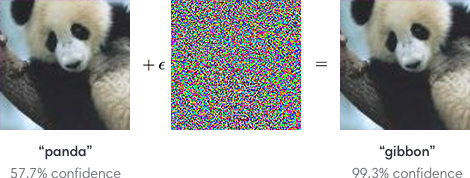
\includegraphics{pics/demo.png}
\caption{}
\end{figure}

In this task, you need to figure out ways to launch one naive
adversarial attack.

    \begin{Verbatim}[commandchars=\\\{\}]
{\color{incolor}In [{\color{incolor}16}]:} \PY{c+c1}{\PYZsh{} Load the ImageNet pretrained model back for adversarial attack}
         \PY{n}{net} \PY{o}{=} \PY{n}{MobileNetV2}\PY{p}{(}\PY{n}{n\PYZus{}class}\PY{o}{=}\PY{l+m+mi}{1000}\PY{p}{)}
         \PY{n}{net} \PY{o}{=} \PY{n}{net}\PY{o}{.}\PY{n}{to}\PY{p}{(}\PY{n}{device}\PY{p}{)}
         
         \PY{k}{if} \PY{n}{device} \PY{o}{==} \PY{l+s+s1}{\PYZsq{}}\PY{l+s+s1}{cuda}\PY{l+s+s1}{\PYZsq{}}\PY{p}{:}
             \PY{n}{net}\PY{o}{.}\PY{n}{load\PYZus{}state\PYZus{}dict}\PY{p}{(}\PY{n}{torch}\PY{o}{.}\PY{n}{load}\PY{p}{(}\PY{l+s+s1}{\PYZsq{}}\PY{l+s+s1}{checkpoint/mobilenet\PYZus{}v2.pth.tar}\PY{l+s+s1}{\PYZsq{}}\PY{p}{)}\PY{p}{)}
         \PY{k}{else}\PY{p}{:}
             \PY{n}{net}\PY{o}{.}\PY{n}{load\PYZus{}state\PYZus{}dict}\PY{p}{(}\PY{n}{torch}\PY{o}{.}\PY{n}{load}\PY{p}{(}\PY{l+s+s1}{\PYZsq{}}\PY{l+s+s1}{checkpoint/mobilenet\PYZus{}v2.pth.tar}\PY{l+s+s1}{\PYZsq{}}\PY{p}{,} \PY{n}{map\PYZus{}location}\PY{o}{=}\PY{l+s+s1}{\PYZsq{}}\PY{l+s+s1}{cpu}\PY{l+s+s1}{\PYZsq{}}\PY{p}{)}\PY{p}{)}
\end{Verbatim}


    \subsubsection{Implement the Attack:}\label{implement-the-attack}

Here you need to add your modification to the input tensor to achieve
the attack. We will count one attack successful if: 1. The visualization
of the noise is merely perceptible (or random pattern) to human eyes.\\
AND\\
2. The MSE of the original input tensor and the modified tensor is below
the threshold.\\
AND\\
3. The network classifies the image to class other than groundtruth.

    \begin{Verbatim}[commandchars=\\\{\}]
{\color{incolor}In [{\color{incolor}17}]:} \PY{k+kn}{import} \PY{n+nn}{torch}\PY{n+nn}{.}\PY{n+nn}{nn}\PY{n+nn}{.}\PY{n+nn}{functional} \PY{k}{as} \PY{n+nn}{F}
         
         \PY{k}{def} \PY{n+nf}{adv\PYZus{}attack}\PY{p}{(}\PY{n}{inputs}\PY{p}{,} \PY{n}{batch\PYZus{}idx}\PY{p}{)}\PY{p}{:}
         \PY{c+c1}{\PYZsh{}     noise = torch.zeros\PYZus{}like(inputs).to(device)}
             \PY{l+s+sd}{\PYZsq{}\PYZsq{}\PYZsq{}}
         \PY{l+s+sd}{    TODO: Implement modification to noise here, achieve the attack}
         \PY{l+s+sd}{    }
         \PY{l+s+sd}{    \PYZsq{}\PYZsq{}\PYZsq{}}
         \PY{c+c1}{\PYZsh{}     net.eval()}
             \PY{n}{epsilon} \PY{o}{=} \PY{l+m+mf}{0.2}
         
             \PY{n}{target} \PY{o}{=} \PY{n}{np}\PY{o}{.}\PY{n}{array}\PY{p}{(}\PY{p}{[}\PY{l+m+mf}{500.}\PY{p}{]}\PY{p}{)}
             \PY{n}{target} \PY{o}{=} \PY{n}{torch}\PY{o}{.}\PY{n}{from\PYZus{}numpy}\PY{p}{(}\PY{n}{target}\PY{p}{)}
             \PY{n}{target} \PY{o}{=} \PY{n}{target}\PY{o}{.}\PY{n}{type}\PY{p}{(}\PY{n}{torch}\PY{o}{.}\PY{n}{LongTensor}\PY{p}{)}
             \PY{n}{inputs} \PY{o}{=} \PY{n}{inputs} \PY{o}{/} \PY{n}{torch}\PY{o}{.}\PY{n}{max}\PY{p}{(}\PY{n}{inputs}\PY{o}{.}\PY{n}{data}\PY{p}{)}
             \PY{n}{inputs}\PY{p}{,} \PY{n}{target} \PY{o}{=} \PY{n}{inputs}\PY{o}{.}\PY{n}{to}\PY{p}{(}\PY{n}{device}\PY{p}{)}\PY{p}{,} \PY{n}{target}\PY{o}{.}\PY{n}{to}\PY{p}{(}\PY{n}{device}\PY{p}{)}
                 
             \PY{n}{inputs}\PY{o}{.}\PY{n}{requires\PYZus{}grad} \PY{o}{=} \PY{k+kc}{True}
             \PY{n}{output} \PY{o}{=} \PY{n}{net}\PY{p}{(}\PY{n}{inputs}\PY{p}{)}
             
             \PY{n}{loss} \PY{o}{=} \PY{n}{F}\PY{o}{.}\PY{n}{nll\PYZus{}loss}\PY{p}{(}\PY{n}{output}\PY{p}{,} \PY{n}{target}\PY{p}{)}
         
         
             \PY{n}{net}\PY{o}{.}\PY{n}{zero\PYZus{}grad}\PY{p}{(}\PY{p}{)}
             \PY{n}{loss}\PY{o}{.}\PY{n}{backward}\PY{p}{(}\PY{p}{)}
         
             \PY{n}{data\PYZus{}grad} \PY{o}{=} \PY{n}{inputs}\PY{o}{.}\PY{n}{grad}\PY{o}{.}\PY{n}{data}
             
             \PY{n}{sign\PYZus{}data\PYZus{}grad} \PY{o}{=} \PY{n}{data\PYZus{}grad}\PY{o}{.}\PY{n}{sign}\PY{p}{(}\PY{p}{)}
             
             \PY{n}{noise} \PY{o}{=} \PY{n}{epsilon}\PY{o}{*}\PY{n}{sign\PYZus{}data\PYZus{}grad}    
             \PY{n}{final} \PY{o}{=} \PY{n}{inputs} \PY{o}{+} \PY{n}{noise}
         
             
             \PY{k}{if} \PY{n}{torch}\PY{o}{.}\PY{n}{mean}\PY{p}{(}\PY{n}{inputs}\PY{o}{\PYZhy{}}\PY{n}{final}\PY{p}{)}\PY{o}{.}\PY{n}{abs}\PY{p}{(}\PY{p}{)} \PY{o}{\PYZlt{}}\PY{o}{=} \PY{l+m+mf}{1e\PYZhy{}3}\PY{p}{:}
                 \PY{n+nb}{print}\PY{p}{(}\PY{l+s+s2}{\PYZdq{}}\PY{l+s+s2}{[INFO] Attack MSE \PYZlt{}= threshold}\PY{l+s+s2}{\PYZdq{}}\PY{p}{)}
             \PY{k}{else}\PY{p}{:}
                 \PY{n+nb}{print}\PY{p}{(}\PY{l+s+s2}{\PYZdq{}}\PY{l+s+s2}{[WARN] Attack MSE \PYZgt{} threshold}\PY{l+s+s2}{\PYZdq{}}\PY{p}{)}
                 
             \PY{n}{inputs\PYZus{}renorm} \PY{o}{=} \PY{p}{(}\PY{n}{inputs} \PY{o}{\PYZhy{}} \PY{n}{inputs}\PY{o}{.}\PY{n}{min}\PY{p}{(}\PY{p}{)}\PY{p}{)} \PY{o}{/} \PY{p}{(}\PY{n}{inputs}\PY{o}{.}\PY{n}{max}\PY{p}{(}\PY{p}{)}\PY{o}{\PYZhy{}}\PY{n}{inputs}\PY{o}{.}\PY{n}{min}\PY{p}{(}\PY{p}{)}\PY{p}{)}
             \PY{n}{noise\PYZus{}renorm} \PY{o}{=} \PY{p}{(}\PY{n}{noise} \PY{o}{\PYZhy{}} \PY{n}{noise}\PY{o}{.}\PY{n}{min}\PY{p}{(}\PY{p}{)}\PY{p}{)} \PY{o}{/} \PY{p}{(}\PY{n}{noise}\PY{o}{.}\PY{n}{max}\PY{p}{(}\PY{p}{)}\PY{o}{\PYZhy{}}\PY{n}{noise}\PY{o}{.}\PY{n}{min}\PY{p}{(}\PY{p}{)}\PY{p}{)}
             \PY{n}{final\PYZus{}renorm} \PY{o}{=} \PY{p}{(}\PY{n}{final} \PY{o}{\PYZhy{}} \PY{n}{final}\PY{o}{.}\PY{n}{min}\PY{p}{(}\PY{p}{)}\PY{p}{)} \PY{o}{/} \PY{p}{(}\PY{n}{final}\PY{o}{.}\PY{n}{max}\PY{p}{(}\PY{p}{)}\PY{o}{\PYZhy{}}\PY{n}{final}\PY{o}{.}\PY{n}{min}\PY{p}{(}\PY{p}{)}\PY{p}{)}
             
             \PY{n}{input\PYZus{}numpy} \PY{o}{=} \PY{n}{inputs\PYZus{}renorm} \PY{p}{[}\PY{l+m+mi}{0}\PY{p}{]}\PY{o}{.}\PY{n}{permute}\PY{p}{(}\PY{l+m+mi}{1}\PY{p}{,} \PY{l+m+mi}{2}\PY{p}{,} \PY{l+m+mi}{0}\PY{p}{)}\PY{o}{.}\PY{n}{cpu}\PY{p}{(}\PY{p}{)}\PY{o}{.}\PY{n}{detach}\PY{p}{(}\PY{p}{)}\PY{o}{.}\PY{n}{numpy}\PY{p}{(}\PY{p}{)}
             \PY{n}{noise\PYZus{}numpy} \PY{o}{=} \PY{n}{noise\PYZus{}renorm} \PY{p}{[}\PY{l+m+mi}{0}\PY{p}{]}\PY{o}{.}\PY{n}{permute}\PY{p}{(}\PY{l+m+mi}{1}\PY{p}{,} \PY{l+m+mi}{2}\PY{p}{,} \PY{l+m+mi}{0}\PY{p}{)}\PY{o}{.}\PY{n}{cpu}\PY{p}{(}\PY{p}{)}\PY{o}{.}\PY{n}{detach}\PY{p}{(}\PY{p}{)}\PY{o}{.}\PY{n}{numpy}\PY{p}{(}\PY{p}{)}
             \PY{n}{final\PYZus{}numpy} \PY{o}{=} \PY{n}{final\PYZus{}renorm} \PY{p}{[}\PY{l+m+mi}{0}\PY{p}{]}\PY{o}{.}\PY{n}{permute}\PY{p}{(}\PY{l+m+mi}{1}\PY{p}{,} \PY{l+m+mi}{2}\PY{p}{,} \PY{l+m+mi}{0}\PY{p}{)}\PY{o}{.}\PY{n}{cpu}\PY{p}{(}\PY{p}{)}\PY{o}{.}\PY{n}{detach}\PY{p}{(}\PY{p}{)}\PY{o}{.}\PY{n}{numpy}\PY{p}{(}\PY{p}{)}
             
             \PY{n}{fig} \PY{o}{=} \PY{n}{plt}\PY{o}{.}\PY{n}{subplot}\PY{p}{(}\PY{l+m+mi}{4}\PY{p}{,}\PY{l+m+mi}{3}\PY{p}{,}\PY{n}{batch\PYZus{}idx}\PY{o}{*}\PY{l+m+mi}{3}\PY{o}{+}\PY{l+m+mi}{1}\PY{p}{)}
             \PY{n}{fig}\PY{o}{.}\PY{n}{imshow}\PY{p}{(}\PY{n}{input\PYZus{}numpy}\PY{p}{)}
             \PY{n}{fig}\PY{o}{.}\PY{n}{text}\PY{p}{(}\PY{l+m+mi}{15}\PY{p}{,} \PY{l+m+mi}{20}\PY{p}{,} \PY{l+s+s1}{\PYZsq{}}\PY{l+s+s1}{original}\PY{l+s+s1}{\PYZsq{}}\PY{p}{,} \PY{n}{bbox}\PY{o}{=}\PY{p}{\PYZob{}}\PY{l+s+s1}{\PYZsq{}}\PY{l+s+s1}{facecolor}\PY{l+s+s1}{\PYZsq{}}\PY{p}{:} \PY{l+s+s1}{\PYZsq{}}\PY{l+s+s1}{white}\PY{l+s+s1}{\PYZsq{}}\PY{p}{,} \PY{l+s+s1}{\PYZsq{}}\PY{l+s+s1}{pad}\PY{l+s+s1}{\PYZsq{}}\PY{p}{:} \PY{l+m+mi}{10}\PY{p}{\PYZcb{}}\PY{p}{)}
             \PY{n}{fig} \PY{o}{=} \PY{n}{plt}\PY{o}{.}\PY{n}{subplot}\PY{p}{(}\PY{l+m+mi}{4}\PY{p}{,}\PY{l+m+mi}{3}\PY{p}{,}\PY{n}{batch\PYZus{}idx}\PY{o}{*}\PY{l+m+mi}{3}\PY{o}{+}\PY{l+m+mi}{2}\PY{p}{)}
             \PY{n}{fig}\PY{o}{.}\PY{n}{imshow}\PY{p}{(}\PY{n}{noise\PYZus{}numpy}\PY{p}{)}
             \PY{n}{fig}\PY{o}{.}\PY{n}{text}\PY{p}{(}\PY{l+m+mi}{15}\PY{p}{,} \PY{l+m+mi}{20}\PY{p}{,} \PY{l+s+s1}{\PYZsq{}}\PY{l+s+s1}{noise}\PY{l+s+s1}{\PYZsq{}}\PY{p}{,} \PY{n}{bbox}\PY{o}{=}\PY{p}{\PYZob{}}\PY{l+s+s1}{\PYZsq{}}\PY{l+s+s1}{facecolor}\PY{l+s+s1}{\PYZsq{}}\PY{p}{:} \PY{l+s+s1}{\PYZsq{}}\PY{l+s+s1}{white}\PY{l+s+s1}{\PYZsq{}}\PY{p}{,} \PY{l+s+s1}{\PYZsq{}}\PY{l+s+s1}{pad}\PY{l+s+s1}{\PYZsq{}}\PY{p}{:} \PY{l+m+mi}{10}\PY{p}{\PYZcb{}}\PY{p}{)}
             \PY{n}{fig} \PY{o}{=} \PY{n}{plt}\PY{o}{.}\PY{n}{subplot}\PY{p}{(}\PY{l+m+mi}{4}\PY{p}{,}\PY{l+m+mi}{3}\PY{p}{,}\PY{n}{batch\PYZus{}idx}\PY{o}{*}\PY{l+m+mi}{3}\PY{o}{+}\PY{l+m+mi}{3}\PY{p}{)}
             \PY{n}{fig}\PY{o}{.}\PY{n}{imshow}\PY{p}{(}\PY{n}{final\PYZus{}numpy}\PY{p}{)}
             \PY{n}{fig}\PY{o}{.}\PY{n}{text}\PY{p}{(}\PY{l+m+mi}{15}\PY{p}{,} \PY{l+m+mi}{20}\PY{p}{,} \PY{l+s+s1}{\PYZsq{}}\PY{l+s+s1}{final}\PY{l+s+s1}{\PYZsq{}}\PY{p}{,} \PY{n}{bbox}\PY{o}{=}\PY{p}{\PYZob{}}\PY{l+s+s1}{\PYZsq{}}\PY{l+s+s1}{facecolor}\PY{l+s+s1}{\PYZsq{}}\PY{p}{:} \PY{l+s+s1}{\PYZsq{}}\PY{l+s+s1}{white}\PY{l+s+s1}{\PYZsq{}}\PY{p}{,} \PY{l+s+s1}{\PYZsq{}}\PY{l+s+s1}{pad}\PY{l+s+s1}{\PYZsq{}}\PY{p}{:} \PY{l+m+mi}{10}\PY{p}{\PYZcb{}}\PY{p}{)}
             
             \PY{k}{return} \PY{n}{final}
\end{Verbatim}


    \begin{Verbatim}[commandchars=\\\{\}]
{\color{incolor}In [{\color{incolor}18}]:} \PY{n}{plt}\PY{o}{.}\PY{n}{figure}\PY{p}{(}\PY{n}{figsize}\PY{o}{=}\PY{p}{(}\PY{l+m+mi}{20}\PY{p}{,}\PY{l+m+mi}{20}\PY{p}{)}\PY{p}{,} \PY{n}{dpi}\PY{o}{=}\PY{l+m+mi}{144}\PY{p}{)}
         \PY{n}{test}\PY{p}{(}\PY{n}{attack}\PY{o}{=}\PY{k+kc}{True}\PY{p}{)}
         \PY{n}{plt}\PY{o}{.}\PY{n}{show}\PY{p}{(}\PY{p}{)}
\end{Verbatim}


    \begin{Verbatim}[commandchars=\\\{\}]
[INFO] Attack MSE <= threshold
Prediction: Alaskan Malamute, Groundtruth: husky
[INFO] Attack MSE <= threshold
Prediction: prayer rug, Groundtruth: jeans
[INFO] Attack MSE <= threshold
Prediction: wallet, Groundtruth: minvan
[INFO] Attack MSE <= threshold
Prediction: mosquito net, Groundtruth: wallet

    \end{Verbatim}

    \begin{center}
    \adjustimage{max size={0.9\linewidth}{0.9\paperheight}}{output_33_1.png}
    \end{center}
    { \hspace*{\fill} \\}
    

    % Add a bibliography block to the postdoc
    
    
    
    \end{document}
